\documentclass[11pt,a4paper]{article}

\usepackage{mypackages}
\usepackage{mycommands}
\usepackage{myenv}
\usepackage{longtable}% TEMPORARY, for the symbol check table

\title{The Topology of Slicing:\\
  A Map-Chain Framework for Slicer Design}
\author{Pierre-Olivier Bolduc}
\date{12 October 2026}

\hypersetup{
  pdftitle={The Topology of Slicing: A Map-Chain Framework for Slicer Design},
  pdfauthor={Pierre-Olivier Bolduc}
}

\begin{document}
  \maketitle

  \begin{abstract}
  Some interruptions of a tool path are chosen by the planner; others are forced by the slicer's structure. We describe a slicer as a chain of maps, from a source through the part and the machine to the built part, and use the chain to locate forced interruptions and design around them. The obstruction is topological: a plan that must visit $c$ path components is interrupted at least $c-1$ times, and the chain identifies the link that supplies them. At the source, every reviewed solid-filling slicer traverses separate layers or surfaces, so its stops grow with resolution. Replacing the source by one connected volume, traversed by a three-dimensional Hilbert curve and carried into the part by optimal transport, gives a continuous path with the prescribed occupation measure on convex parts. In a computational prototype, it makes no stops on convex parts, where a layered raster's stops roughly double with resolution; on non-convex parts, a source split into near-convex pieces trades a fixed number of transitions for bounded excursions. At the machine, the components are the posture sheets of the robot's safe configurations, and a slicer that fixes the tool path first inherits the posture switches that path forces. Reversing the construction order gives kinematics-first slicing, in which the sheets guide the source split. On a three-link planar arm among obstacles, it makes the single posture reset required by the bound in a sampled availability model, while a geometry-first baseline makes two. The two constructions serve as demonstrations of the framework: one counting argument bounds both stops and posture switches, and in both a source split matched to the components attains the minimum.
\end{abstract}

  \section{Introduction}
\label{sec:introduction}

A slicer turns a part into machine motion, and on the way it makes several decisions: which source to traverse, in what order, how to place it in the part, how to turn the tool path into machine motion, and how that motion deposits material. Most slicers bundle these decisions into one algorithm, so two slicers differ in several decisions at once, and a limit that many of them share can go unnoticed because it lies in a decision that none of them varies. Separating the decisions lets slicers be compared one decision at a time, lets each guarantee and failure be traced to the decision that supplies it, and lets alternatives be constructed by making one decision differently. This paper develops that separation as a framework, the map chain, and demonstrates it on interruptions.

The motion a slicer produces is rarely one continuous stroke. The flow stops between layers, and a robot may have to change posture partway through. Some of these interruptions are chosen by a planner and could be planned away; others are forced by the structure of the slicer. We use the framework to find which stage forces them and how to design a slicer that avoids them. Figure~\ref{fig:teaser} shows a tool path built this way.

\begin{figure}[!ht]
  \centering
  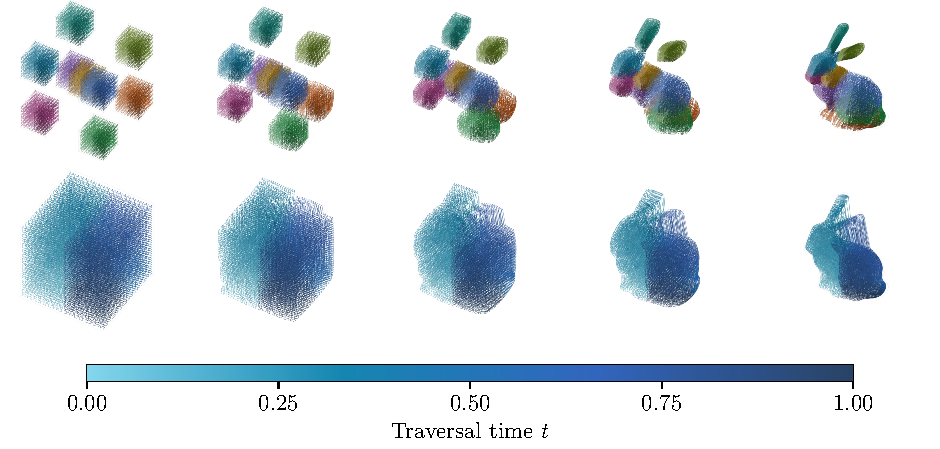
\includegraphics[width=\textwidth]{figures/bunny_transport_decomposition.pdf}
  \caption{The first application of the framework: a connected volume, not a stack of layers, as the source. Top: a decomposed source of nine cubes, each transported onto one piece of the Stanford bunny; each piece has its own colour, light at its start and dark at its end. Bottom: a Hilbert path through one cube ($32\,768$ cells) is moved into the bunny by optimal transport, coloured by traversal time. Intermediate shapes are drawn for illustration. The visiting order comes from the cubes, and the shape, including the ears, from the map alone.}
  \label{fig:teaser}
\end{figure}

On a simple cylinder, a layered raster must stop between layers, and the count roughly doubles each time the resolution doubles (Section~\ref{main:evidence}). Each stop of the material flow can leave a seam, and in some processes a stop is especially costly: it can cut reinforcing fibre in continuous-fibre printing \cite{fang2024exceptional}, cause a restart defect in wire-arc deposition \cite{ding2014toolpath}, or weaken the bond in concrete printing \cite{tay2019timegap}. Better paths within each layer remove some stops, but not those between layers. A robot shows the same pattern one stage later: when obstacles split its safe postures into separate families, some tool paths cannot be followed without a posture reset, however good the inverse kinematics.

\paragraph{The map-chain framework.}
We treat a slicer as a chain of maps, from a source representation through the part and the machine to the built part (Section~\ref{main:chain}). The framework makes three contributions: (i)~a common description for comparing slicers, in which each slicer is a choice of links and of their construction order, so that slicers can be compared link by link and their shared choices become visible (Section~\ref{main:families}); (ii)~composition rules, by which coverage, continuity, containment, and implementation error compose from link to link, so that each guarantee or failure can be traced to the link that supplies it (Section~\ref{main:compose}); and (iii)~a design procedure, in which replacing a link choice that existing slicers hold fixed, or changing the construction order, defines a new construction whose surviving guarantees and new obligations the rules state. Forced interruptions are topological, because each continuous stretch of motion remains within one path component of the space it moves in: a plan that must visit $c$ components is interrupted at least $c-1$ times, and the chain locates the link that supplies the components (Section~\ref{main:source}). We demonstrate the procedure on two shared choices that, in the slicing literature we review, force interruptions at two different links; the resulting constructions show what the framework makes visible, not its full extent.

\paragraph{First application: changing the source.}
Every reviewed solid-filling slicer traverses a source of separate layers or surfaces. Separating the source from the traversal makes the alternative visible: one connected volume, traversed directly. The \emph{transported Hilbert path} (Section~\ref{main:construction}) orders a cube with a three-dimensional Hilbert curve and carries it into the part by optimal transport, so that the traversal fixes the visiting order and the geometry map the shape. On convex parts the path is continuous and has exactly the prescribed occupation measure; on non-convex parts, decomposing the source into near-convex pieces meets containment up to each piece's hull gap.

\paragraph{Second application: changing the construction order.}
Every reviewed slicer builds the tool path first, and that path then fixes how often the robot must switch between families of safe postures. Separating the geometry map from the lift makes the alternative visible: build admissible machine motion first and derive the tool path from it through forward kinematics. This requires a new map from the source into configurations. In \emph{kinematics-first slicing} (Section~\ref{main:next}), guarantees and obligations trade places: static feasibility holds by construction, while coverage and the prescribed deposition density become obligations, met by a source split that the posture families guide.

\paragraph{Scope.}
All evidence is computational. The volumetric experiments end at the geometric tool path, and no part has been printed. In the robot experiment, feasibility is static, and the separation of posture families and the optimality of the switch counts hold only in a sampled model. Physical posture resets and material deposition are not modelled. Section~\ref{main:outlook} returns to these boundaries.

\paragraph{Research prototype and reproducibility.}
The research prototype, saved reference results, and figure-generation code are available at \url{https://github.com/pobol2/Topology-of-Slicing}.

  \section{The map chain as a slicer design framework}
\label{main:chain}

\subsection{The map chain}
Figure~\ref{fig:main-chain} reads a slicer as a sequence of decisions. A slicer first chooses a \emph{source} $\Xs$, the space in which the path is designed: a stack of slices, a family of surface patches, or a volume. A \emph{traversal} ${\vect{\upxi}}\colon[0,1]\to\Xs$ then decides the order in which the source is visited over normalised deposition time $t\in[0,1]$. A \emph{geometry map} $\Phi\colon\Xs\to\Omega$ places each source point in the part $\Omega\subset\mathbb R^3$, which produces the tool path ${\vect{x}}\colon[0,1]\to\Omega$. Finally, a \emph{lift} $\Psi_{\mathrm{g}}$, where $\mathrm{g}$ marks the geometry-first construction order, turns the tool path into the joint path ${\vect{q}}\colon[0,1]\to\Qs$ in the machine's configuration space $\Qs$, and the \emph{process} $\Theta$ turns that motion into the built part $\widehat\Omega\subset\mathbb R^3$, where a hat marks a realised or computed approximation of the unhatted object:
\begin{equation}
  \label{eq:main-chain}
  {\vect{x}}=\Phi\circ{\vect{\upxi}},\qquad {\vect{q}}=\Psi_{\mathrm{g}}[{\vect{x}}],\qquad
  \widehat\Omega=\Theta[{\vect{q}}].
\end{equation}
Here ${\vect{x}}(t)=\Phi({\vect{\upxi}}(t))$, so the geometry map acts pointwise; square brackets indicate that the lift and the process take whole paths as inputs.

\begin{figure}[htbp]
  \centering
  \tikzsetnextfilename{map-chain}
  \begin{tikzpicture}[box/.style={draw,rounded corners,fill=black!4,minimum width=2.3cm,minimum height=0.9cm,text height=2.2ex,text depth=0.6ex,align=center},arr/.style={-{Stealth},thick}]
    \node[box] (s) at (0,0) {Time $[0,1]$};
    \node[box] (v) at (3.3,0) {Source $\Xs$};
    \node[box] (g) at (6.6,0) {Part $\Omega$};
    \node[box] (q) at (9.9,0) {Machine $\Qs$};
    \node[box] (p) at (13.2,0) {Material $\widehat\Omega$};
    \draw[arr] (s)--node[above] {${\vect{\upxi}}$}(v);
    \draw[arr] (v)--node[above] {$\Phi$}(g);
    \draw[arr] (g)--node[above] {$\Psi_{\mathrm{g}}$}(q);
    \draw[arr] (q)--node[above] {$\Theta$}(p);
  \end{tikzpicture}
  \caption{The map chain, shown schematically through its underlying spaces. Traversal and geometry act pointwise; the arrows into machine motion and material act on whole paths.}
  \label{fig:main-chain}
\end{figure}

The chain also decides how much material goes where. Suppose the traversal spends its time in the source according to a distribution $\mu_{\Xs}$, a probability measure on $\Xs$, and the geometry map sends $\mu_{\Xs}$ to the prescribed distribution $\mu_\Omega$ on the part. Then the tool path spends its deposition time according to $\mu_\Omega$. Writing $f_\#\mu$ for the image of a distribution $\mu$ under a map $f$, and $\lambda^1$ for the uniform distribution of time on $[0,1]$ (the superscript denotes dimension),
\begin{equation}
  \label{eq:main-measure}
  {\vect{\upxi}}_\#\lambda^1=\mu_{\Xs},\quad \Phi_\#\mu_{\Xs}=\mu_\Omega
  \quad\Longrightarrow\quad
  {\vect{x}}_\#\lambda^1=\mu_\Omega .
\end{equation}
With constant flow, time shares are material shares, so the identity states what it means for a path to cover the part with the right amount of material. Graded density needs no separate link: any chain can carry it through $\mu_{\Xs}$ or $\mu_\Omega$.

A planar slicer illustrates every link. Its source is the set of $N$ separate cross-sections, $\Xs=\bigsqcup_{j=1}^N\Xs_j$, each a planar region labelled by its layer. Its traversal zigzags within each slice and visits the slices in order, the geometry map lifts each slice to its height, the lift turns the tool path into machine motion, and the process deposits material. The resulting distribution lives on $N$ slices, so the process must fill the gaps between them. Definition~\ref{def:cms} in Appendix~\ref{sec:cms-spaces} states the chain formally.

\subsection{How guarantees compose}
\label{main:compose}
The chain is useful because guarantees attach to links and compose from one link to the next; Appendix~\ref{sec:cms-composition} states the rules with proofs (Proposition~\ref{prop:composition}) and tabulates the resulting guarantees (Table~\ref{tab:cms-guarantees}). Four rules carry the arguments of this paper.
\begin{itemize}
  \item \emph{Coverage.} Exact distributions compose exactly, as in \eqref{eq:main-measure}; a distribution error at one link passes through the next link's modulus of continuity and adds to that link's own error.
  \item \emph{Continuity.} Moduli of continuity compose, and ${\vect{x}}=\Phi\circ{\vect{\upxi}}$ can be discontinuous only where the traversal is, or where it meets a discontinuity of $\Phi$.
  \item \emph{Containment.} If each link maps into the region that the next accepts, so does the composition; this keeps a tool path in the part and a joint path in the admissible configurations.
  \item \emph{Error propagation.} Implementation errors, such as solver tolerances, propagate in the same way, which is why the finite-order bounds of Section~\ref{main:convex} have one term per link.
\end{itemize}
Repairing one link does not repair another: denser sampling cannot fix a wrong geometry map, and a better lift cannot fill missing coverage. Each failure therefore has an address: a disconnected source forces transitions, a geometry map can tear the path or leave a non-convex part, a lift can switch branches near a singularity \cite{zhang2021singularity}, and the process can leave gaps. This paper stops before the process: the composed guarantees describe paths and occupation measures, not a manufactured part.

\paragraph{Designing with the chain.}
The same decomposition gives a procedure for deriving new slicers. Read an existing construction link by link and identify a choice that it holds fixed; replace that choice, or change the order in which the links are constructed; then use the composition rules to determine which guarantees survive and which become obligations for the remaining links. A replaced link must establish its own certificates, and a new order may need new maps rather than a rearrangement of the old ones (Section~\ref{main:next}). Sections~\ref{main:construction} and~\ref{main:next} apply this procedure to the two choices that the review below exposes.

\subsection{Existing slicers as link choices}
\label{main:families}
Table~\ref{tab:main-families} compares the reviewed slicer families as design choices. Each row gives the source as the family traverses it, the links it changes relative to the planar chain, and whether it constructs the tool path or the machine motion first. A row lists a family's characteristic change; families often combine changes, and S$^3$-Slicer, the scalar-field method, and the neural slicer target multi-axis machines and so also change $\Psi_{\mathrm{g}}$ \cite{zhang2022s3,dai2018support,liu2024neural}. The kinematics-first row uses $\Psi_{\mathrm{k}}$, a map from the source into machine configurations defined in Section~\ref{main:next}.

\begin{papertable}
  \begin{papertabular}{>{\raggedright\arraybackslash}p{3.2cm}>{\raggedright\arraybackslash}p{4.0cm}>{\raggedright\arraybackslash}p{1.6cm}>{\raggedright\arraybackslash}p{1.0cm}>{\raggedright\arraybackslash}p{3.9cm}}
    \toprule
    Family & Source $\Xs$ & Links changed & Order & Examples \\
    \midrule
    Planar (reference) & $N$ flat layers & -- & Geom. & \cite{prusaslicer} \\
    Adaptive layer height & $N$ flat layers, variable spacing & $\Xs$ & Geom. & \cite{dolenc1994slicing,pandey2003slicing,alexa2017optimal} \\
    Within-layer continuous & $N$ flat layers & ${\vect{\upxi}}$ & Geom. & \cite{zhao2016fermat,bedel2022closed,gupta2019continuous} \\
    Curved layers & $N$ curved layers & $\Phi$ & Geom. & \cite{etienne2019curvi,zhang2022s3} \\
    Multi-axis & $N$ layers or surfaces & $\Psi_{\mathrm{g}}$ & Geom. & \cite{chalvin2020layer,schmitz2021robot,zhang2021singularity} \\
    Scalar-field & $N$ level surfaces & $\Xs$, $\Phi$ & Geom. & \cite{dai2018support} \\
    Trivariate & Parameter volume, visited surface by surface & $\Xs$, $\Phi$ & Geom. & \cite{ezair2018volumetric} \\
    Neural mappings & $N$ learned curved layers & $\Phi$ & Geom. & \cite{liu2024neural,dutta2025implicit} \\
    Surface paths & $N$ surface patches & $\Xs$, ${\vect{\upxi}}$ & Geom. & \cite{zhong2023acap} \\
    Vase mode & One surface (a single wall) & $\Xs$, ${\vect{\upxi}}$, $\Phi$ & Geom. & \cite{prusaslicer} \\
    \midrule
    Transported Hilbert path & One solid volume, or $N$ volumes if decomposed & $\Xs$, ${\vect{\upxi}}$, $\Phi$ & Geom. & This paper, Sections~\ref{main:construction}--\ref{main:evidence} \\
    Kinematics-first & $c$ patches, one per posture sheet & $\Xs$, $\Psi_{\mathrm{k}}$ & Kin. & This paper, Section~\ref{main:next} \\
    \bottomrule
  \end{papertabular}
  \caption{Slicer families compared as design choices: the links each changes relative to the planar chain, and its construction order. The source column is the source as it is actually traversed; the order column records whether the tool path (Geom.) or the machine motion (Kin.) is constructed first. Every reviewed family above the rule builds geometry first, and every solid-filling one traverses separate layers or surfaces. The table is representative, not exhaustive. Below the rule are the two constructions of this paper: the first changes the source; the second changes the construction order, and its map $\Psi_{\mathrm{k}}$ into configurations takes the place of both $\Phi$ and $\Psi_{\mathrm{g}}$.}
  \label{tab:main-families}
\end{papertable}

Families that look very different agree on two choices: all build geometry first, and every solid-filling family traverses its source as $N$ separate pieces. Representing the solid as a volume does not change the second choice, because representing a volume is not traversing it. The trivariate method parameterises a volume but visits it surface by surface \cite{ezair2018volumetric}, and volumetric frame fields \cite{chermain2025atomizer} and implicit neural fields \cite{dutta2025implicit} likewise describe the solid as a volume but print it as layers or surfaces. Two alternatives are therefore absent from the reviewed methods, and they motivate the two applications of this paper: traversing a connected volume, and constructing the machine motion before the tool path. The first concerns the source, whose disconnection carries a cost that no other link can pay back, as the next subsection shows; the second concerns the order of construction (Section~\ref{main:next}).

\subsection{A topological consequence: pieces force transitions}
\label{main:source}
The composition rules give upper bounds: they say where a path can be interrupted. The topology of the source supplies a matching lower bound. Let the source have $N$ separate pieces, each receiving positive deposition time. Any traversal that is continuous except at finitely many times then makes at least $N-1$ \emph{transitions} between pieces, in whatever order it visits them (Proposition~\ref{prop:topology-transitions}, Appendix~\ref{sec:topology}). A better order shortens the moves but cannot reduce their number. Section~\ref{main:next} applies the same counting argument at the machine link.

A transition is an event in the source, not yet a stop; its effect on the machine depends on the later links. Where two mapped pieces touch, a transition can be crossed continuously in the part, as between adjacent patches. When the geometry map is continuous on each piece and the mapped pieces do not touch, a transition becomes a break of the tool path. A break forces a \emph{stop}: a break occupies no deposition time, so the machine crosses it with a travel move during which the flow is switched off. For layers, every transition is a stop, because distinct layers lie at least the layer spacing $h$ apart (Corollary~\ref{cor:topology-propagation}).

The stop count of a layered slicer therefore grows with resolution: a part needs at least one stop fewer than it has layers, so for a fixed part height, halving the layer spacing approximately doubles the lower bound, and disconnected cross-sections can add further transitions.

Since these stops originate in the source, the design procedure changes the source, and the simplest replacement for a solid is a single connected volume. The composition rules state the cost: a connected source removes forced transitions only if a traversal can visit it continuously and a geometry map can carry it into the part without tearing it apart again. Section~\ref{main:construction} meets these two obligations.

  \section{First application: changing the source}
\label{main:construction}

The first application follows the design procedure of Section~\ref{main:chain} step by step. A disconnected source forces transitions (Section~\ref{main:source}); choosing the unit cube, a connected volume, removes that structural cause. The composition rules then state what the remaining links must supply. The tool path $x=\Phi\circ\xi$ is continuous only if both the traversal and the geometry map are, and by \eqref{eq:main-measure} it has the prescribed occupation measure only if
\begin{equation}
  \label{eq:main-volume-obligations}
  \xi_\#\lambda^1=\lambda^3,\qquad \Phi_\#\lambda^3=\mu_\Omega ,
\end{equation}
where $\lambda^3$ is uniform volume on the cube. The traversal must therefore be a continuous, measure-preserving curve through the cube, and the geometry map must be a continuous map that pushes uniform volume onto $\mu_\Omega$. A space-filling curve meets the first obligation exactly, and optimal transport meets the second, with continuity under the convexity assumptions below. The resulting \emph{transported Hilbert path}, or transported path for short, gives each map a single job: the traversal orders, and the geometry map shapes. The construction ends at the tool path: the lift and the process remain abstract links of the chain.

\subsection{Construction: Hilbert orders, transport shapes}
The traversal is the three-dimensional Hilbert curve $\Hil$ \cite{hilbert1891,sagan1994,bader2013}. It visits every point of the cube continuously, spends equal time in equal volumes, and keeps points visited at nearby times close together. At a finite order $m$ it visits the centres $u_1,\dots,u_n$ of $n=8^m$ cells, consecutive cells sharing a face \cite{haverkort2017}; Appendix~\ref{sec:vsfc-hilbert} establishes its measure preservation, locality, and finite-order estimates. Here the geometry map $\Phi$ is chosen as the optimal-transport map. Among all maps that send uniform volume in the cube to the target distribution $\mu_\Omega$, it minimises the mean squared displacement \cite{brenier1991,peyre2019computational}. The transported path is
\begin{equation}
  \label{eq:main-vsfc}
  x(t)=\Phi\bigl(\Hil(t)\bigr).
\end{equation}

\begin{figure}[tb]
  \centering
  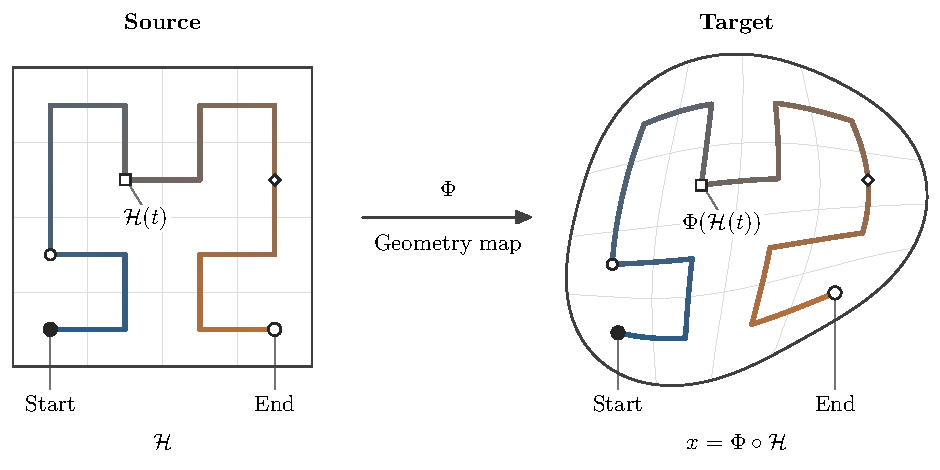
\includegraphics[width=\textwidth]{figures/hilbert_transport.pdf}
  \caption{Hilbert orders, transport shapes. A numerical two-dimensional illustration of the volumetric construction: an order-two Hilbert traversal $\mathcal H$ in the source square (left) is carried into the target by a smooth approximation of the geometry map $\Phi$ (right), computed from an entropically regularised quadratic optimal-transport solve. Matching colours and marker shapes indicate corresponding traversal times; the visiting order is inherited from the source.}
  \label{fig:hilbert-transport}
\end{figure}

Composition gives $x_\#\lambda^1=\Phi{}_\#\lambda^3=\mu_\Omega$; when transport is continuous, the composed path is continuous as well. Figure~\ref{fig:hilbert-transport} illustrates the construction numerically in two dimensions, and Figure~\ref{fig:teaser} (top) illustrates the construction on the Stanford bunny. Its distinction is to transport a traversed volume while preserving the prescribed occupation measure: earlier manufacturing uses of Hilbert curves traverse layers or deposition surfaces \cite{bertoldi1998domain,papacharalampopoulos2018path}, while curved-layer, multi-axis, and neural slicers deform layers \cite{etienne2019curvi,zhang2022s3,liu2024neural}.

\subsection{Guarantees on convex parts}
\label{main:convex}
The Hilbert curve is continuous, so the transported path is continuous wherever the transport map is. Optimal transport always delivers the prescribed distribution, but it need not be continuous: a map that sends a cube onto a shape with a hole may have to tear. Convex targets avoid this. If the part is compact and convex with nonempty interior, and the target density is bounded above and below by positive constants, the transport map is H\"older continuous on the closed cube \cite{caffarelli1992,jhaveri2022regularity}; Appendix~\ref{app:proofs-convex-transport} explains why these assumptions suffice. We call these assumptions the \emph{convex setting}.

In the convex setting, the ideal transported path is continuous and has the prescribed occupation measure, $x_\#\lambda^1=\mu_\Omega$; Appendix~\ref{sec:vsfc-certificates} derives this (Theorem~\ref{thm:vsfc-guarantees}(ii)) together with the finite-order bounds below. Physically, the nozzle never has to break off and travel: the path has no stop, and the time it spends in each region matches the prescription.

At a finite Hilbert order $m$, the guarantee becomes a bound. Waypoints $\hat x_i$ that lie within $\varepsilon$ of $\Phi(u_i)$ satisfy, for constants $\beta\in(0,1]$ and $C_\Phi$ (Theorem~\ref{thm:vsfc-guarantees}(i)),
\begin{equation}
  \label{eq:main-bounds}
  \text{covering radius}\leq C_\Phi2^{-\beta m}+\varepsilon,\qquad
  \text{step length}\leq C_\Phi2^{-\beta m}+2\varepsilon .
\end{equation}
The two terms belong to different links. A finer Hilbert order shrinks the first; only a more accurate geometry map shrinks the second. The constants are not known for a computed map, which is why the computation below supplies a bound of its own.

Outside the convex setting, the guarantee is absent rather than refuted: transport still delivers the prescribed distribution, but no theorem makes it continuous. Implementing the construction also requires computing the map, which brings its own certificates and its own gaps.

\subsection{Implementation: semi-discrete transport}
\label{main:semidiscrete}
The waypoints are computed by semi-discrete optimal transport between the part and the finite Hilbert curve \cite{aurenhammer1998minkowski,merigot2011multiscale,levy2015numerical}. The order-$m$ curve is the discrete measure $\nu_m=n^{-1}\sum_i\delta_{u_i}$, one unit of time per site, and the part carries the continuous target $\mu_\Omega=\rho\,dy$, which may be graded. For weights $\psi\in\mathbb R^n$, the \emph{Laguerre cell} of site $u_i$ is the part of $\Omega$ that is power-nearest to it,
\begin{equation}
  \label{eq:main-laguerre}
  L_i(\psi)=\bigl\{y\in\Omega:\ \|y-u_i\|^2-\psi_i\leq\|y-u_j\|^2-\psi_j\ \text{for all }j\bigr\}.
\end{equation}
The cells always tile $\Omega$. The solver adjusts $\psi$ until every cell carries its site's share of the target, up to solver tolerance,
\begin{equation}
  \label{eq:main-equal-mass}
  \mu_\Omega\bigl(L_i(\psi)\bigr)=\tfrac1n\qquad(i=1,\dots,n),
\end{equation}
which makes the map sending each $L_i$ to $u_i$ the optimal transport from $\mu_\Omega$ to $\nu_m$ \cite{aurenhammer1998minkowski,peyre2019computational}. Each Hilbert site is finally replaced by the density-weighted centroid of its cell,
\begin{equation}
  \label{eq:main-centroid}
  \hat x_i=n\int_{L_i(\psi)}y\,\rho(y)\,dy ,
\end{equation}
and the waypoints are visited in Hilbert order. A Hilbert site thus labels a cell of the part rather than serving as a waypoint, and the waypoint is the centre of mass of that cell. On the cube with uniform density, each cell is the Hilbert cell and $\hat x_i=u_i$: the construction is the identity, as it should be.

This construction controls, cell by cell, what the ideal map is meant to control; Appendix~\ref{sec:vsfc-semidiscrete} proves its distribution, order, and containment properties (Proposition~\ref{prop:sd-mass}) and the hull-gap bounds used below.
\begin{itemize}
  \item \emph{Cell mass.} Every waypoint stands for the same mass $1/n$ of the target, matching the equal time that the Hilbert curve spends in each cell. No target sample is drawn and none is deleted.
  \item \emph{A computable distribution bound.} Sending each cell's mass to its own centroid moves no mass farther than the largest cell diameter $D_m=\max_i\operatorname{diam}L_i(\psi)$, so the waypoints match the target to within $W_\infty\leq D_m$. Unlike $\varepsilon$ in \eqref{eq:main-bounds}, $D_m$ is measured for every computed path.
  \item \emph{Order.} Each centroid stays power-nearest to its own site, so the waypoints inherit the Hilbert labels without reordering.
\end{itemize}

Three things are not controlled, and the third becomes the turning point of the construction. First, how fast $\hat x_i$ approaches $\Phi(u_i)$ is not certified, so the step bound in \eqref{eq:main-bounds} remains conditional. Second, equal cell mass is not waypoint-density accuracy: regions thinner than a cell are not resolved (Proposition~\ref{prop:sd-mass}(iii)). Third, equal mass says nothing about containment. On a convex part each clipped cell is convex, so every centroid and every segment between consecutive centroids lies in the part. On a non-convex part, two mechanisms break this: a cell straddling a reentrant corner is clipped into disconnected portions whose combined centroid can lie in the empty region between them, and two cells with centroids inside the part can be joined by a segment that crosses a hole. Figure~\ref{fig:containment-repair} (Section~\ref{main:evidence}) shows both on computed paths.

\subsection{Repair: a volumetric source in several pieces}
\label{main:decomposed}
The chain assigns this failure to the geometry map, not the source: the cube is still connected, and the excursions arise where cells are clipped by holes and reentrant edges. The repair therefore stays within the first application: it restores the geometry map's convexity assumption, or nearly so, while keeping the source volumetric. Instead of one cube, the source becomes $k$ cubes, each transported onto a convex or near-convex piece of the part. Every piece is still filled by a path that runs through its volume; what changes is that the part now receives several piece paths instead of one. How far each piece may be from convex is measured by a single quantity.

\paragraph{A geometric guarantee for near-convex domains.}
For a compact domain $K$, let $\delta_K=\sup_{z\in\operatorname{conv}(K)}\dist(z,K)$ be its \emph{convex-hull gap}: how far its convex hull reaches beyond it. Centroids of cells contained in $K$, and straight segments joining them, lie in its convex hull, hence within distance $\delta_K$ of $K$ (Proposition~\ref{prop:sd-hull-gap}). This bound needs no transport regularity and recovers exact containment when $K$ is convex. It bounds excursion depth only.

\paragraph{The decomposed source.}
Given a partition of the part into $k$ convex or near-convex pieces $\Omega_1,\dots,\Omega_k$, the source is $k$ cubes, one per piece, and the Hilbert traversal and semi-discrete transport are applied independently to each (Figure~\ref{fig:teaser}, bottom). Each piece receives its share $w_j=\mu_\Omega(\Omega_j)$ of deposition time, and its path leaves it by at most its own hull gap $\delta_j$, with exact containment for convex pieces (Corollary~\ref{cor:sd-piece-hull-gap}).

Two kinds of excursion must now be kept apart. A piece path can leave its \emph{assigned piece}, by at most $\delta_j$; such an excursion may enter a neighbouring piece and so remain inside the part. Or it can leave the \emph{whole object}, which is the failure that decomposition is meant to remove. The hull-gap bound controls the first directly; it controls the second only where the region within $\delta_j$ of a piece lies inside the part.

\paragraph{The remaining tradeoff.}
Decomposition reintroduces separate pieces into the source, so Proposition~\ref{prop:topology-transitions} forces at least $k-1$ transitions between piece paths. Unlike the $N$ layers of a layered slicer, $k$ is set by the partition of the part, not by the Hilbert order, so the count does not grow as the resolution is refined. Sequencing the pieces, and hence executing these transitions, is outside the scope of this paper.

  \section{Evaluating the first application}
\label{main:evidence}

The framework makes three predictions about the first application, each naming a link: changing the source removes the transitions between layers; the failures that remain belong to the geometry map; and decomposition repairs them up to each piece's hull gap. A computational demonstration tests them and also measures the distribution control that separating order from shape is meant to provide. Its scope is stated in Section~\ref{sec:introduction}.

The implementation computes the semi-discrete map of Section~\ref{main:semidiscrete} with the solver of Geogram \cite{levy2015numerical,kitagawa2019convergence}, on parts meshed into tetrahedra \cite{si2015tetgen}, solving coarse to fine. The five parts are a cylinder, a sphere, a solid torus, an L-bracket with a reentrant edge, and a complex part consisting of a block with several holes and a boss (genus three). Every run, at orders $m=4,5,6$ ($4096$ to $262\,144$ waypoints), met the equal-mass condition to a relative tolerance of $10^{-6}$. A stop is counted wherever a path would have to be executed as travel: for the layered raster baseline, each travel move; for the transported path, each maximal \emph{exterior run} of segments that leave the part. Steps longer than five times the mean are reported separately as \emph{jumps}. Appendix~\ref{sec:implementation} gives the meshing, solver settings, and acceptance checks; Appendix~\ref{sec:experiments-setup} defines the metrics and the layered baseline; and Table~\ref{tab:experiments-geometries} in Appendix~\ref{sec:experiments-geometries} reports all fifteen runs.

\paragraph{A connected source removes the stops on convex parts.}
Figure~\ref{fig:layer-stops} shows the mechanism on a cube at order two. The decisive count is the number of stops between layers, which Proposition~\ref{prop:topology-transitions} forces. On the cylinder, a layered raster makes 13, 27, and 57 of them at orders 4, 5, and 6, roughly doubling with the number of layers, while the transported path has no layers to stop between and no exterior run at any tested order (Table~\ref{tab:main-stops}). That zero follows by construction on a convex part; beyond it, the path has no jump, and its longest step shrinks with the order. Changing the source thus removes a limit that grows with every refinement of the layered chain.

\begin{figure}[tb]
  \centering
  \includegraphicsorbox{figures/cube_layer_interruptions.pdf}{0.85\textwidth}{5.5cm}
  \caption{Layer changes on a cube at order two (64 waypoints). (a) Layered raster on the same cell centres: dashed red segments mark the three layer changes, each requiring a stop. (b) Computed transported path: it changes height throughout, so there is no layer boundary to stop at, and it has no exterior run. Colour indicates traversal time, from light (start, circle) to dark (end, square). Stop counts under refinement are in Table~\ref{tab:main-stops}.}
  \label{fig:layer-stops}
\end{figure}

% Written by python -m mapchain tables from results/evaluation/raster and results/evaluation/whole_part.
\begin{papertable}
  \begin{papertabular}{lrrr}
    \toprule
    & \multicolumn{2}{c}{Layered raster} & Transported path \\
    \cmidrule(lr){2-3}\cmidrule(lr){4-4}
    Part & Between layers & All travel & Exterior runs \\
    \midrule
    Cylinder & 13 / 27 / 57 & 97 / 419 / 2029 & 0 / 0 / 0 \\
    Sphere & 13 / 27 / 57 & 101 / 371 / 1533 & 0 / 0 / 0 \\
    Torus & 5 / 11 / 23 & 69 / 271 / 1163 & 1 / 53 / 241 \\
    L-bracket & 3 / 9 / 19 & 3 / 19 / 19 & 53 / 224 / 836 \\
    Complex part & 5 / 11 / 23 & 37 / 155 / 586 & 95 / 323 / 1103 \\
    \bottomrule
  \end{papertabular}
  \caption{Stops at Hilbert orders 4 / 5 / 6. Most raster travel lies within layers, where a better in-layer planner could remove some of it; only the stops between layers are forced.}
  \label{tab:main-stops}
\end{papertable}


\paragraph{The distribution is controlled cell by cell.}
Every accepted path assigns each waypoint the same target mass, so each waypoint stands for one Hilbert time block. On the convex parts the computable bound $d^{(m)}$ roughly halves with each order, from $0.120$ to $0.065$ and $0.035$ on the cylinder, and the covering radius follows. This is consistent with the $2^{-\beta m}$ term of \eqref{eq:main-bounds}, though three orders do not determine $\beta$.

\paragraph{On non-convex parts, the failures lie in the geometry map and persist under refinement.}
As the framework predicts, the source stays connected and the failures come from non-convex clipped cells (Figure~\ref{fig:containment-repair}). On the L-bracket, cells near the reentrant edge straddle the empty region between the arms and their centroids lie in it. On the torus at order four, every waypoint is inside the part, but one segment joins two interior centroids across the hole, which is also how most exterior segments of the complex part arise; Appendix~\ref{sec:experiments-resolution} separates the two mechanisms. Refinement lowers the fraction of exterior segments on the L-bracket and the complex part, but not the deepest excursions (Table~\ref{tab:experiments-geometries}): cells clipped by holes and reentrant edges stay large, and on the L-bracket $d^{(m)}$ stays near $0.85$, because refinement does not make the target convex. The cost is real: the torus has fewer exterior runs than the raster has travel moves, but the L-bracket and complex part have more (Table~\ref{tab:main-stops}). This persistence motivates decomposition.

\begin{figure}[tb]
  \centering
  \includegraphicsorbox{figures/nonconvex_containment_decomposition.pdf}{\textwidth}{7cm}
  \caption{Containment failures and their repair, computed at order four (plan views; top row L-bracket, bottom row torus; red marks the path outside the part). Left: whole-part paths (4096 waypoints). Middle: close-up of the boxed region; thick segments join consecutive waypoints (dots). On the L-bracket, an exterior run passes through a waypoint in the empty region beside the reentrant corner. On the torus, the single exterior segment joins two interior waypoints across the hole. Right: piece paths, with one colour per piece: the two convex boxes of the L-bracket at order four, and eight automatic torus pieces at order three (4096 waypoints in total, the whole-part budget; Appendix~\ref{sec:experiments-torus-figure}). No piece-path segment leaves the part.}
  \label{fig:containment-repair}
\end{figure}

\paragraph{Decomposition restores containment up to each piece's hull gap.}
We apply the same traversal and solver independently to the two boxes of the L-bracket and to an automatic partition of the torus into eight pieces; all ten local solves pass. The results match the two kinds of excursion of Section~\ref{main:decomposed}. Against each \emph{assigned piece}, the bound holds: the two convex boxes give full containment, as Proposition~\ref{prop:sd-hull-gap} guarantees (Figure~\ref{fig:containment-repair}, top right), and the automatic torus pieces, which are not exactly convex, have segments that leave their own piece, but every excursion stays below that piece's computed hull-gap bound (Table~\ref{tab:decomposition}). Against the \emph{whole object}, these crossings enter neighbouring pieces, not empty space: at the same budget of $32\,768$ waypoints, the whole-part path has 99 segments leaving the torus, while the piece paths have none, with similar coverage (Table~\ref{tab:torus-whole-vs-pieces}). These are sampled measurements with numerical hull-gap bounds, not containment certificates; Appendix~\ref{sec:experiments-pieces-independent} gives the partition procedure, the hull-gap evaluation, and the same-budget protocol.

% Written by python -m mapchain tables from results/evaluation/pieces/torus_whole_vs_pieces.json.
\begin{papertable}
  \begin{papertabular}{lrrrrrrr}
    \toprule
    Path / domain & Inside & Ext.\ seg. & Ext.\ length & Depth & Coverage & CV & Radius \\
    \midrule
    Whole / torus & 99.98\% & 0.30\% & 0.51\% & $0.0317$ & $0.981$ & $0.392$ & $0.0244$ \\
    Pieces / torus & 100.00\% & 0.00\% & 0.00\% & $0.0000$ & $0.978$ & $0.405$ & $0.0200$ \\
    Pieces / assigned & 98.40\% & 5.21\% & 3.11\% & $0.0232$ & -- & -- & -- \\
    \bottomrule
  \end{papertabular}
  \caption{Torus at the same budget: one whole-part path and eight piece paths, $32\,768$ waypoints each. \emph{Torus} measures against the whole object, \emph{assigned} against each path's own piece. ``Inside'' is the percentage of waypoints inside the evaluation domain; ``Ext.\ seg.'' and ``Ext.\ length'' are the percentages of exterior segments and exterior path length. Depth is the deepest sampled excursion; radius is the sampled covering radius. Distances are in normalised units; coverage and the coefficient of variation (CV) are defined in Appendix~\ref{sec:experiments-setup}. See Appendix~\ref{sec:experiments-torus-comparison} for the comparison protocol.}
  \label{tab:torus-whole-vs-pieces}
\end{papertable}


Decomposition thus trades a growing count for a fixed one: it brings back $N$ source components, independent of resolution, in exchange for containment up to each piece's hull gap. The first application kept the usual order of construction, geometry first and machine second. The second changes that order, because the next source of forced interruptions lies in the machine.
\FloatBarrier

  \section{Second application: changing the construction order}
\label{main:next}

The first application replaced one link. The second demonstrates the other move of the design procedure: changing the order in which the links are constructed, which redistributes guarantees and obligations among them. A connected source can still lead to interruptions at the machine. If obstacles divide the robot's safe postures into separate families, a tool path that passes between their regions forces sheet switches, by the same counting argument, and which link fixes that count depends on the construction order. Every reviewed slicer constructs the tool path first. Geometry-first slicing fixes ${\vect{x}}=\Phi\circ{\vect{\upxi}}$, which certifies the occupation measure through $\Phi$, and then seeks a lift ${\vect{q}}=\Psi_{\mathrm{g}}[{\vect{x}}]$ that follows it. Robot-aware methods do plan with machine constraints, but they take a geometric path or geometric elements as input \cite{chalvin2020layer,schmitz2021robot,zhang2021singularity,huang2018choreo}, so obstacles, singularities, and posture changes are resolved for a geometry that is already fixed. Reversing the order is not a permutation of the same maps: $\Psi_{\mathrm{g}}$ lifts a prescribed tool path, whereas a machine-first construction needs a new map $\Psi_{\mathrm{k}}\colon\Xs\to\Qfree$ from the source into admissible configurations, and derives the tool path through forward kinematics (FK; Figure~\ref{fig:kin-order}):
\begin{equation}
  \label{eq:kinematicsfirst}
  {\vect{q}}=\Psi_{\mathrm{k}}\circ{\vect{\upxi}},\qquad {\vect{x}}=\FK\circ {\vect{q}},
\end{equation}
where $\Qfree\subseteq\Qs$ is the set of admissible configurations (within joint limits and free of collisions) and $\FK\colon\Qs\to\mathbb R^3$ returns the tool position. Guarantees and obligations trade places. Static feasibility holds by construction, while coverage and the prescribed occupation measure, ${\vect{x}}_\#\lambda^1=\mu_\Omega$, which geometry-first obtains from $\Phi$, become obligations. Configuration-first coverage exists in robotics: Yang et~al.\ \cite{yang2020coverage} plan coverage through configuration-space cells to minimise discontinuities. The framework adds the prescribed deposition measure and the link to source decomposition.

\begin{figure}[tbp]
  \centering
  \begin{minipage}[t]{0.48\textwidth}
    \centering
    \begin{tikzcd}[column sep=1.8cm, row sep=1.1cm, ampersand replacement=\&]
      \vect{\upxi} \arrow[r, "{\Phi\circ(\cdot)}"] \arrow[dr, dashed, thin] \& \vect{x} \arrow[d, "{\Psi_{\mathrm{g}}[\cdot]}"] \\
      \& \vect{q}
    \end{tikzcd}

    {\small(a) Geometry first\par}
  \end{minipage}\hfill
  \begin{minipage}[t]{0.48\textwidth}
    \centering
    \begin{tikzcd}[column sep=1.8cm, row sep=1.1cm, ampersand replacement=\&]
      \vect{\upxi} \arrow[r, "{\Psi_{\mathrm{k}}\circ(\cdot)}"] \arrow[dr, dashed, thin] \& \vect{q} \arrow[d, "{\FK\circ(\cdot)}"] \\
      \& \vect{x}
    \end{tikzcd}

    {\small(b) Kinematics first\par}
  \end{minipage}

  \caption{The two construction orders. (a) Geometry first: construct the tool path, then lift it to machine motion. (b) Kinematics first: construct admissible machine motion, then derive the tool path through forward kinematics; covering the target $\Omega$ with the prescribed measure remains an obligation. Vertices denote paths. An arrow labelled $f\circ(\cdot)$ applies $f$ pointwise to a path; square brackets denote whole-path input. The dashed diagonals give ${\vect{q}}=\Psi_{\mathrm{g}}[\Phi\circ{\vect{\upxi}}]$ in (a) and ${\vect{x}}=\FK\circ\Psi_{\mathrm{k}}\circ{\vect{\upxi}}$ in (b).}
  \label{fig:kin-order}
\end{figure}

\paragraph{The density obligation.}
\label{sec:kinematics-density}
Let $\Psi_{\mathrm{k}}$ map into a regular submanifold of $\Qfree$ on which $\FK$ is injective in a regular chart, and let $\mu_{\Qs}={\vect{q}}_\#\lambda^1$ be the distribution of deposition time over configurations. The joint path deposits the target exactly when
\[
  \FK_\#\mu_{\Qs}=\mu_\Omega .
\]
Because $\FK$ stretches volume unevenly, a uniform distribution over configurations need not give uniform deposition. Where patches overlap, the target mass is partitioned first and each patch carries its share; multiple preimages must be summed rather than treated as one branch.

\subsection{Posture sheets guide the source split}
\label{sec:kin-sheets}
Once the order is reversed, the robot rather than the target can guide how the source is split, as the part's convexity guided it in the first application (Section~\ref{main:decomposed}). Call the path components of the safe fibre space $\{({\vect{y}},{\vect{q}})\in\Omega\times\Qfree:\FK({\vect{q}})={\vect{y}}\}$ \emph{sheets}. These sheets are related to t-connectivity \cite{wenger1991freeworkspace} and aspects \cite{borrel1986aspects}. A \emph{sheet switch} occurs at a time $t$ where the one-sided limits $({\vect{x}}(t^-),{\vect{q}}(t^-))$ and $({\vect{x}}(t^+),{\vect{q}}(t^+))$ lie in different sheets; a discontinuity within one sheet is not counted. A \emph{posture reset} is a discrete posture change with the flow off; it may be a sheet switch or an in-sheet reset. A continuous stretch of a lifted path stays in one sheet, so a switch is the robot's analogue of a source transition. If one region is reachable only in sheet~1 and another only in sheet~2, every passage of the tool path from the first to the second forces a switch, whatever lift is chosen.

The construction makes the split explicit. (1) Cover $\Omega$ by patches $U_j\subseteq\Omega$, each inside the projection of one sheet. (2) Construct and validate a continuous safe lift of $U_j$ into $\Qfree$ within that sheet. (3) Choose assigned regions $\Omega_j\subseteq U_j$ that cover $\Omega$ with pairwise $\mu_\Omega$-null overlaps, and give piece $j$ its target-mass share $w_j=\mu_\Omega(\Omega_j)>0$ and conditional measure $\mu_\Omega(\,\cdot\mid\Omega_j)$. (4) Traverse each assigned region with its own source piece, using the prepared lift on $U_j$, and visit each piece once.

\begin{proposition}[Sheets force switches; patches attain the minimum]
  \label{prop:sheets-switches}
  Let $\supp\mu_\Omega=\Omega$, where $\supp$ denotes the support of a measure, and let $c$ be the fewest sheets whose projections cover $\Omega$. (i) Every plan with ${\vect{x}}_\#\lambda^1=\mu_\Omega$, finitely many discontinuities, and safe one-sided limits makes at least $c-1$ switches. (ii) If $\Omega$ is covered by $c$ patches $U_j$, with assigned regions $\Omega_j\subseteq U_j$ that partition the target measure as above, and each assigned region is traversed with its conditional measure and time share $w_j$ by a continuous safe lift in one sheet, visiting each assigned region once attains $c-1$. In particular, if two sheets are necessary and two such patches cover $\Omega$, one switch is necessary and sufficient.
\end{proposition}
Appendix~\ref{app:kin-proof} gives the proof. Two distinctions bound the claim. Sheet coverage is not lift existence: a sheet whose projection covers a patch need not supply a continuous lift over it, so the patch lifts are hypotheses to validate. And a counted switch is an event in deposition time, whereas the physical repositioning between postures, with the flow off, is a separate collision-free motion that must be planned and checked. For a fixed path, the same argument fixes the count: with two sheets whose closed projections admit continuous sections, the minimum number of switches equals the number of alternations between the region reached only by the first sheet and the region reached only by the second. A geometry-first slicer inherits this count from its path; a better lift cannot lower it, just as a better order of source pieces cannot lower the number of transitions.

\subsection{A three-link experiment}
\label{sec:kinematics-example}
\paragraph{Setup.}
A planar arm with three revolute joints and unit links deposits on an annular sector among three disk obstacles (Figure~\ref{fig:sheets-3r}(a)). Its safe fibre space is sampled at seven radii; in this sampled availability model, three sheets are necessary and sufficient to cover $\Omega$, so $c=3$. Sampling rules out neither a connection through an unsampled passage nor availability at unsampled radii. Both pipelines use $4^m$ waypoints at orders $m=3,4,5$ and two target densities, uniform and a gradient. \emph{Geometry-first}, our baseline, follows the order-$m$ Hilbert path over the whole chart, solving constrained inverse kinematics at each collocation point, warm-started from the previous solution; when the current sheet fails, it switches to the sheet that stays available longest along the path. \emph{Kinematics-first} follows the construction of Proposition~\ref{prop:sheets-switches}. A one-time preparation places handoff curves between consecutive sheets and stores a certified joint-pose map on each of three patches (Figure~\ref{fig:sheets-3r}(b)). Each request divides the target mass among the assigned regions, traverses each region with its own source piece, and reads joint poses from the stored maps without solving inverse kinematics; consecutive regions are joined at a handoff point, where a posture reset occurs (Figure~\ref{fig:sheets-3r}(d)). The \emph{reset count} is the number of observed discrete posture changes; the \emph{coverage error} is the largest distance from a target grid to the sampled depositing path; the \emph{density error} is the total-variation distance between target shares and waypoint shares on $4\times8$ area bins. Appendix~\ref{app:kin-setup} gives the geometry, sampling, preparation, mass allocation, certification, and timing protocol.

\paragraph{Results.}
Kinematics-first made two sheet switches and no in-sheet resets in all six requests, attaining the bound $c-1=2$ (Table~\ref{tab:sheets-3r-results}). Geometry-first made four sheet switches in every request, the minimum for its fixed Hilbert path in the sampled availability model: the path crosses between regions served by different sheets more often than the cover requires. In two gradient-density requests it also made an additional in-sheet reset, where its warm-started lift lost a branch inside a sheet that still covered the region, an instance of the gap between sheet coverage and lift existence. The excess over $c-1$ is thus a property of the geometry-first path and its lift, not of the solver tolerances, and the reduction to two comes from the sheet-guided split of the source. Coverage errors are comparable and shrink with the order. For uniform density, the geometry-first density error is zero because its waypoints are the Hilbert cell centres, whereas kinematics-first gives each patch a whole number of source columns, and this rounding of mass shares produces its density error; for gradient density the two errors are close. Kinematics-first keeps a sampled clearance of $0.033$ to $0.038$, because its patch maps maximise clearance, while geometry-first's warm-started solutions stay at the imposed margin of $10^{-3}$; its connectors to and from the handoff points add at most $11\%$ of tool travel. After a one-time preparation of $21.0$~s, kinematics-first planned and certified each request in at most $0.17$~s, against $9.3$ to $35.8$~s for geometry-first. The advantage comes from reusing the prepared maps instead of solving inverse kinematics per request, and is not exclusive to kinematics-first construction: a geometry-first planner could also cache inverse maps.

% Written by python -m mapchain tables from results/kinematics/results.json and benchmark.json.
\begin{papertable}
  \begin{papertabular}{llrrrrrrrr}
    \toprule
    & & \multicolumn{2}{c}{Resets} & \multicolumn{2}{c}{Coverage error} & \multicolumn{2}{c}{Density error} & \multicolumn{2}{c}{Planning (s)} \\
    \cmidrule(lr){3-4}\cmidrule(lr){5-6}\cmidrule(lr){7-8}\cmidrule(lr){9-10}
    Density & $m$ & G & K & G & K & G & K & G & K \\
    \midrule
    Uniform & 3 & 4 & 2 & 0.265 & 0.291 & 0.000 & 0.031 & 10.92 & 0.015 \\
    & 4 & 4 & 2 & 0.133 & 0.145 & 0.000 & 0.070 & 18.03 & 0.055 \\
    & 5 & 4 & 2 & 0.066 & 0.069 & 0.000 & 0.029 & 35.79 & 0.168 \\
    \addlinespace
    Gradient & 3 & 4 & 2 & 0.475 & 0.570 & 0.172 & 0.158 & 9.25 & 0.016 \\
    & 4 & 4$+$1 & 2 & 0.250 & 0.217 & 0.043 & 0.068 & 17.04 & 0.055 \\
    & 5 & 4$+$1 & 2 & 0.129 & 0.136 & 0.031 & 0.032 & 29.59 & 0.168 \\
    \bottomrule
  \end{papertabular}
  \caption{Three-link comparison of geometry-first (G) and kinematics-first (K) at $4^m$ waypoints. Resets are observed discrete posture changes: sheet switches, plus in-sheet resets after $+$ where the warm-started lift loses its branch inside a sheet. Coverage error is in target units; density error is total variation of original-waypoint shares on $4\times8$ area bins. Planning time is the median time to plan and certify one request. Kinematics-first also has a one-time preparation of $21.0$~s; the shared fibre analysis ($15.8$~s) is excluded for both.}
  \label{tab:sheets-3r-results}
\end{papertable}


In this example, the change of order placed each obligation where the construction could meet it: density through the source split, up to rounding; clearance in the prepared patch maps; and most of the work in a one-time preparation. These observations hold for one arm, obstacle layout, and implementation, not as general performance guarantees. Admissibility is static, with joint rates and dynamics unchecked, and the posture resets are counted but not planned or certified as physical motions. As in the first application, the forced interruptions are counted by the path components at one link, and a source split matched to those components attains the minimum.

\begin{figure}[H]
  \centering
  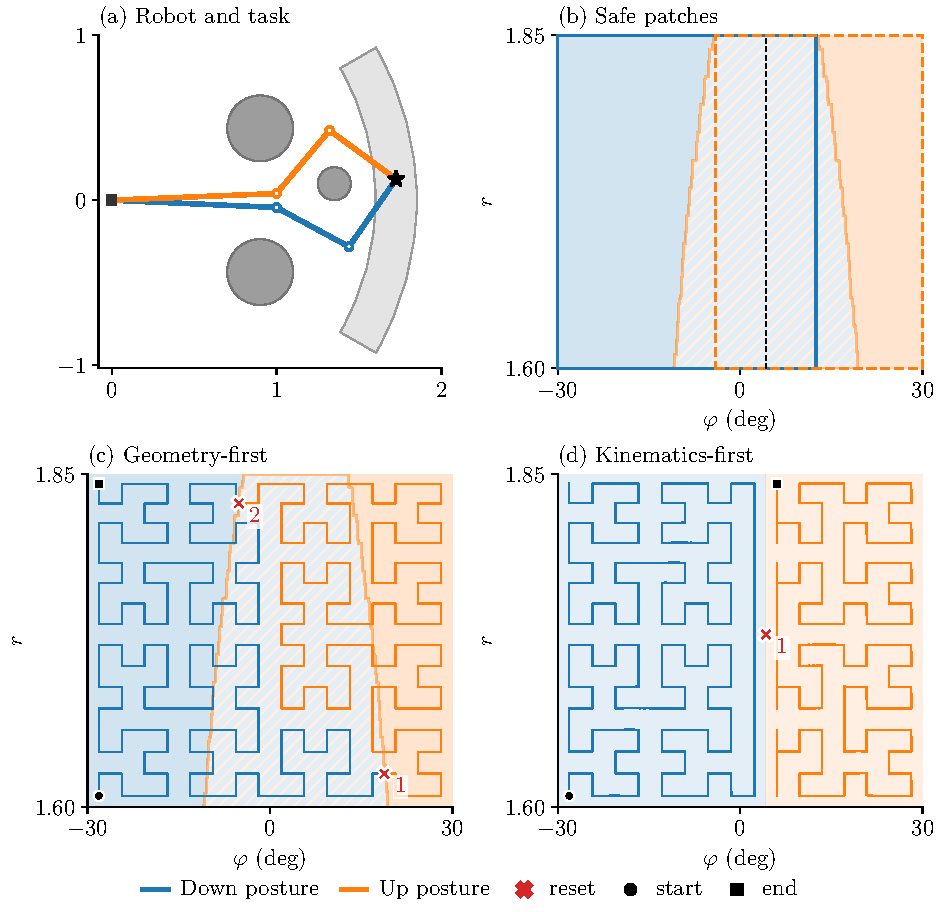
\includegraphics[width=\textwidth]{figures/three_link_posture_comparison.pdf}
  \caption{Three-link experiment at order five with uniform density; colours mark the sheets used. (a) Arm, obstacles, target sector, and the postures available at one tool point. (b) Robot-guided split: sampled availability of the three sheets over the chart, in each sheet's colour where it alone is available and in the mix of the two colours where two are, the certified patch domains $U_j$ (outlines), and the handoff curves (dashed). (c) Geometry-first path, coloured by sheet over the same availability shading, with four sheet switches. (d) Kinematics-first path, shaded by assigned region: each region is completed once, with one sheet switch at each of the two handoff points. Red crosses mark discrete, uncertified posture resets. The certified connectors to and from the handoff points are not drawn.}
  \label{fig:sheets-3r}
\end{figure}
\FloatBarrier

  \section{Outlook}
\label{main:outlook}

The two applications demonstrate the framework; they do not exhaust it. Both were obtained by the design procedure of Section~\ref{main:chain}, and we see three directions in which it extends.

\paragraph{Unexplored link choices.}
Table~\ref{tab:main-families} is sparse. Every reviewed family builds geometry first and treats the process $\Theta$ as fixed, and the two constructions of this paper fill only two new cells. Sources can lie between a stack of layers and one volume, for instance a few connected pieces chosen to match the part and the machine at once. Traversals of a connected source need not be Hilbert curves; other curves trade locality, smoothness, and turning differently. Construction orders can interleave the links rather than fix one first; a process-aware order, for example, could let thermal or curing constraints in $\Theta$ shape the source split as the posture sheets did here. Each of these choices comes with its own obligations, and the composition rules say in advance what they are.

\paragraph{Lower bounds that combine several links.}
The two bounds of this paper each count components at one link, but obstructions can arise at several at once, as when a part decomposed into $N$ near-convex pieces is printed by a robot whose safe postures form $c$ sheets. Unless the source pieces align with the sheets, we expect the true minimum to be counted by the components of a combined space of source pieces and sheets that a continuous stretch can occupy together, and to exceed both $N-1$ and $c-1$. Stating and proving such bounds, and building sources that attain them, would turn the counting argument from a diagnosis of one link into a design rule for the whole chain.

\paragraph{Uses beyond deposition.}
Any process that covers a region with a prescribed measure along a machine-executed path has the same chain, including machining (material removed), inspection (sensor dwell), and spraying and welding (coating or heat input). Each has its own forced interruptions, such as tool retractions, re-fixturing, and torch restarts, and its own machine with posture sheets.

  \section{Conclusion}
\label{main:scope}

Forced interruptions in slicing are topological (Section~\ref{sec:introduction}): the map chain shows which link supplies the components and what a construction that changes that link, or the order of construction, must guarantee in its place.

The two applications find these components at two different links. In the first, they are the pieces of the source. A connected volume as the source removes them and leaves two obligations: a continuous measure-preserving traversal and a continuous geometry map. A Hilbert curve and optimal transport meet these obligations on convex parts. On non-convex parts, decomposing the source repairs the remaining failures up to each piece's hull gap, at the cost of a fixed number of transitions. In the second application, the components are the robot's posture sheets. Building admissible machine motion first lets the sheets guide the source split, and patches with continuous safe lifts, each visited once, attain the minimum.

Neither algorithm alone shows that stops and posture switches obey one counting argument, attained in both cases by a source split matched to the components; the framework does. Maps that stay inside non-convex parts, sequencing of decomposed pieces, and smoothing that preserves containment and respects machine dynamics are the natural next steps, alongside the directions of Section~\ref{main:outlook}. Slicing has been developed by improving paths within a fixed chain. The chain itself---its links, their order, and the components each one supplies---is where the forced limits of a slicer are set, and where new slicers can be designed.

  \label{main-text-end}

  \clearpage
  \appendix

  \section{Framework and interruption guarantees}
\label{sec:cms}

This appendix supports the framework claims of Section~\ref{main:chain}: that a slicer is a chain of maps, that guarantees compose from link to link, and that a disconnected source forces transitions. Subsection~\ref{sec:cms-spaces} fixes the spaces, the deposition-time convention, and the formal definition of a geometry-first map chain. Subsection~\ref{sec:cms-composition} states and proves the composition rules. Subsection~\ref{sec:topology} proves the transition bound for disconnected sources and its propagation into tool-path, machine, and deposition interruptions.

\subsection{Spaces, paths, and the map chain}
\label{sec:cms-spaces}

Let $\Omega\subset\mathbb{R}^3$ be compact, with target deposition measure $\mu_\Omega$. All measures are probability measures, and $f_\#\eta(A)=\eta(f^{-1}(A))$ is the pushforward of $\eta$ by a measurable map $f$. The target measure may be volumetric or live on lower-dimensional sets such as layers. Let $\Qs$ be the configuration space of the machine \cite{lavalle2006}, with the tool-position forward-kinematics map
\begin{equation}
  \label{eq:cms-forward-kinematics}
  \FK:\Qs\to\mathbb{R}^3,\qquad x=\FK\circ q.
\end{equation}
The static admissible set $\Qfree\subseteq\Qs$ encodes joint limits, a prescribed singularity margin, and avoidance of fixed obstacles.

\paragraph{Deposition time.}
Time $t\in I=[0,1]$ is normalised deposition time, and $\lambda^1$ is the uniform probability measure on $I$. For a space $M$, $\Paths{M}$ denotes the paths $I\to M$ that are continuous on the pieces of a finite partition of $I$, with one-sided limits at the breakpoints; $C^0(I,M)\subseteq\Paths{M}$. Physical execution crosses each discontinuity with a non-deposition travel move, which takes machine time but no deposition time. The traversal $\xi$, tool path $x$, and joint path $q$ share the time parameter.

\begin{definition}[Map chain]
  \label{def:cms}
  For a prescribed target $(\Omega,\mu_\Omega)$, a geometry-first map chain is a tuple
  $(\Xs,\mu_{\Xs},\xi,\Phi,\Psi_g)$, where:
  \begin{itemize}
    \item $\Xs$ is a compact manifold with boundary, or a finite disjoint union of such manifolds, of dimension at most three;
    \item $\mu_{\Xs}$ is a probability measure on $\Xs$;
    \item $\xi\in\Paths{\Xs}$ is the traversal, satisfying $\xi_\#\lambda^1=\mu_{\Xs}$;
    \item $\Phi:\Xs\to\Omega$ is a measurable geometry map, satisfying $\Phi_\#\mu_{\Xs}=\mu_\Omega$;
    \item $\Psi_g:\mathcal{D}\to\Paths{\Qs}$ is a configuration lift on a declared domain of paths $\mathcal{D}\subseteq\Paths{\Omega}$, satisfying
          \begin{equation}
            \label{eq:cms-lift}
            \FK\circ\Psi_g[x]=x\qquad\text{for all }x\in\mathcal{D}.
          \end{equation}
  \end{itemize}
\end{definition}
The lift applies only when $x$ has finitely many discontinuities, which is not automatic for a measurable $\Phi$ (Subsection~\ref{sec:vsfc-ot}); applicability of the lift and static admissibility therefore require separate certificates. With both pushforward conditions, \eqref{eq:main-measure} gives the tool path the occupation measure $\mu_\Omega$. The process operator $\Theta$, which maps a joint path to a manufactured set for a fixed process and protocol, is left abstract.

Definition~\ref{def:cms} and the certificates below describe the geometry-first order, in which the tool path is built and then lifted. The kinematics-first construction of Section~\ref{main:next} is not a permutation of these maps: it introduces a new map $\Psi_k$ from the source into $\Qfree$ and derives the tool path through forward kinematics \eqref{eq:kinematicsfirst}, so static feasibility becomes a certificate of $\Psi_k$, while the occupation measure becomes the density obligation stated there.

The lift acts on whole paths because, for an $n$-joint arm at a regular value of $\FK$, the fibre $\FK^{-1}(x)$ is locally $(n-3)$-dimensional \cite{burdick1989}: no configuration in it is canonical, and singularities can prevent a globally continuous inverse branch \cite{gottlieb1988robots,pavesic2017topologist,zhang2021singularity}. A lift is therefore selected along the whole path \cite{kazerounian1988global,chalvin2020layer,yang2020coverage}.

\paragraph{The planar chain.}
In the planar chain, $D_k$ is the cross-section at height $z_k$, and the label $k$ keeps the slices apart in the source even though the solid is connected. The ideal source measure is $\mu_{\Xs}=\sum_kw_k\bar\lambda_{D_k}$, with $w_k\geq0$ the time share of layer $k$ and $\bar\lambda_{D_k}$ the normalised area measure on $D_k\times\{k\}$. A finite zigzag only approximates this area measure; taking $\mu_{\Xs}$ to be the normalised occupation measure of the zigzag centreline instead gives an exact chain for the finite raster.

\subsection{Certificates that compose}
\label{sec:cms-composition}

A \emph{certificate} is a property of one stage alone, on a specified domain. Five kinds are used:
\begin{itemize}
  \item \emph{Coverage:} a pushforward identity, or a measure error bounded in $W_\infty$.
  \item \emph{Regularity:} a modulus of continuity $\omega_f(\delta)=\sup_{d(a,a')\leq\delta}d(f(a),f(a'))$.
  \item \emph{Discontinuity:} the set $\Sigma(f)$ of discontinuity points, or a certified set containing it.
  \item \emph{Containment:} a region containing the image of the stage.
  \item \emph{Stability:} a uniform implementation error $\|\hat f-f\|_\infty\leq\varepsilon_f$, measured in the target space of the stage.
\end{itemize}
For probability measures on a compact metric space, $W_\infty$ \cite{champion2008infinity} is the smallest $r$ such that some coupling moves no mass farther than $r$. For paths with discontinuities, regularity certificates hold on each continuous piece.

\begin{proposition}[Composition rules]
  \label{prop:composition}
  Let $f\colon A\to B$ and $g\colon B\to C$ be measurable stages between compact metric spaces and $\mu$ a probability measure on $A$, with $\nu$ and $\kappa$ target probability measures on $B$ and $C$.
  \begin{enumerate}[label=(\roman*)]
    \item \emph{Coverage.} $W_\infty\bigl((g\circ f)_\#\mu,\kappa\bigr)\leq\omega_g\bigl(W_\infty(f_\#\mu,\nu)\bigr)+W_\infty(g_\#\nu,\kappa)$. In particular, exact pushforward certificates compose exactly.
    \item \emph{Regularity.} $\omega_{g\circ f}\leq\omega_g\circ\omega_f$.
    \item \emph{Discontinuity.} $\Sigma(g\circ f)\subseteq\Sigma(f)\cup f^{-1}\bigl(\Sigma(g)\bigr)$.
    \item \emph{Containment.} If $f(A)\subseteq B'$ and $g(B')\subseteq C'$, then $(g\circ f)(A)\subseteq C'$.
    \item \emph{Stability.} If implementations $\hat f,\hat g$ satisfy $\lVert\hat f-f\rVert_\infty\leq\varepsilon_f$ on $A$ and $\lVert\hat g-g\rVert_\infty\leq\varepsilon_g$ on $\hat f(A)$, with $\omega_g$ taken on $f(A)\cup\hat f(A)$, then $\lVert\hat g\circ\hat f-g\circ f\rVert_\infty\leq\varepsilon_g+\omega_g(\varepsilon_f)$.
  \end{enumerate}
\end{proposition}
\begin{proof}
  For (i), an optimal $W_\infty$ coupling of $f_\#\mu$ and $\nu$ exists on compact spaces \cite{champion2008infinity}; push it forward by $g\times g$ and apply the triangle inequality for $W_\infty$. Items (ii)--(iv) are immediate from the definitions, and (v) follows from $\lVert\hat g\circ\hat f-g\circ\hat f\rVert_\infty+\lVert g\circ\hat f-g\circ f\rVert_\infty$.
\end{proof}
Rule (iii) is an upper bound; Proposition~\ref{prop:topology-transitions} gives the matching lower bound for disconnected sources. Rule (ii) multiplies H\"older exponents. Repairing one stage does not repair another: denser sampling cannot fix a wrong geometry map, and a better lift cannot fill missing coverage.

\begin{corollary}[$W_\infty$ gives a covering radius]
  \label{cor:cms-covering-radius}
  If $W_\infty(\nu,\mu_\Omega)\leq r$, then every point of $\supp\mu_\Omega$ lies within distance $r$ of $\supp\nu$.
\end{corollary}
\begin{proof}
  An optimal coupling matches almost every target point to a point of $\supp\nu$ within distance $r$. Distance to this closed set is continuous, and every neighbourhood of a point of $\supp\mu_\Omega$ has positive mass, so the bound extends to all of $\supp\mu_\Omega$.
\end{proof}
With $\supp\mu_\Omega=\Omega$, one coupling bound therefore controls both the distribution of deposition time and the covering radius of the path.

Because $\Psi_g$ acts on paths, its certificates take a different form: a nondecreasing transfer function $T_\Psi$, such that an input path with modulus at most $\omega$ lifts to a joint path with modulus at most $T_\Psi(\omega)$; a set $B_\Psi$ of branch-switch times, with $\Sigma(q)\subseteq\Sigma(x)\cup B_\Psi$; and a region $U\subseteq\Omega$ whose admitted paths lift into $\Qfree$. A pointwise section with Lipschitz constant $L_\Psi$ has $T_\Psi(\omega)=L_\Psi\,\omega$. Table~\ref{tab:cms-guarantees} assembles the certificates; replacing a stage changes only its column.

\begin{papertable}
  \begin{papertabular}{>{\raggedright\arraybackslash}p{2.0cm}
      >{\raggedright\arraybackslash}p{2.3cm}
      >{\raggedright\arraybackslash}p{2.4cm}
      >{\raggedright\arraybackslash}p{3.0cm}
      >{\raggedright\arraybackslash}p{5.0cm}}
    \toprule
    Property & $\xi$ & $\Phi$ & $\Psi_g$ & Resulting guarantee \\
    \midrule
    Coverage &
    $\xi_\#\lambda^1=\mu_{\Xs}$ &
    $\Phi_\#\mu_{\Xs}=\mu_\Omega$ &
    $\FK\circ\Psi_g[x]=x$ &
    $x_\#\lambda^1=\mu_\Omega$ \\
    Regularity &
    $\omega_\xi$ &
    $\omega_\Phi$ &
    $T_\Psi$ &
    $\omega_q\leq T_\Psi(\omega_\Phi\circ\omega_\xi)$ \\
    Discontinuity &
    $\Sigma(\xi)$ &
    $\Sigma(\Phi)$ &
    $B_\Psi$ &
    $\Sigma(q)\subseteq\Sigma(\xi)$\newline
    $\quad\cup\xi^{-1}(\Sigma(\Phi))\cup B_\Psi$ \\
    Static feasibility &
    -- &
    $\Phi(\Xs)\subseteq U$ &
    $\Paths{U}\to\Paths{\Qfree}$ &
    $q\in\Paths{\Qfree}$ \\
    \bottomrule
  \end{papertabular}
  \caption{Certificates along the geometry-first chain. Each resulting guarantee is a property of the tool path $x$ or joint path $q$, or of the occupation measure of $x$, and depends only on the certificates in its own row; none describes a manufactured part. Feasibility is with respect to the static set $\Qfree$ only.}
  \label{tab:cms-guarantees}
\end{papertable}


\subsection{Transitions of disconnected sources}
\label{sec:topology}

Suppose the source is a finite disjoint union of compact connected components,
\begin{equation}
  \label{eq:topology-source}
  \Xs=\bigsqcup_{k=1}^{N}\Xs_k.
\end{equation}
Planar layers give at least one component per layer; curved layers \cite{etienne2019curvi,zhang2022s3}, separate surfaces \cite{zhong2023acap}, and parameterisation patches \cite{ezair2018volumetric} give others. The components are those of the source, not of the part: the images $\Phi(\Xs_k)$ can touch or overlap in $\Omega$. Four kinds of interruption must be kept apart.

\begin{definition}[Interruptions]
  \label{def:topology-interruptions}
  \leavevmode
  \begin{itemize}
    \item A \emph{source interruption} is a discontinuity of the traversal $\xi$; a \emph{transition} is a source interruption at which $\xi$ passes from one component to another.
    \item A \emph{tool-path interruption} is a discontinuity of $x=\Phi\circ\xi$.
    \item A \emph{machine interruption} is a discontinuity of the joint path $q=\Psi_g[x]$.
    \item A \emph{deposition interruption} is a stop of the material flow during physical execution.
  \end{itemize}
\end{definition}
The first three occur in deposition time; the last occurs in machine time, which also includes travel moves.

\begin{proposition}[Source-component transitions]
  \label{prop:topology-transitions}
  Let $\Xs$ be as in \eqref{eq:topology-source}, let $\xi\in\Paths{\Xs}$ satisfy $\xi_\#\lambda^1=\mu_{\Xs}$, and suppose $\mu_{\Xs}(\Xs_k)>0$ for every $k$.
  \begin{enumerate}[label=(\roman*)]
    \item The traversal $\xi$ has at least $N-1$ transitions, whatever the order in which it visits the components.
    \item Suppose $\Phi$ is continuous on each component. At a transition $t_i$, the tool path $x=\Phi\circ\xi$ has the one-sided limits $x(t_i^\pm)=\Phi(\xi(t_i^\pm))$, and it is discontinuous at $t_i$ unless
          \begin{equation}
            \label{eq:topology-identify}
            \Phi\bigl(\xi(t_i^-)\bigr)=\Phi\bigl(\xi(t_i^+)\bigr).
          \end{equation}
  \end{enumerate}
\end{proposition}
\begin{proof}
  (i) Let $0=t_0<\cdots<t_m=1$ be a partition on whose open pieces $\xi$ is continuous. The image of each piece is connected, so it lies in one component; label the piece by that component. Each component has positive mass, so by $\xi_\#\lambda^1=\mu_{\Xs}$ it is visited for a positive time, and its label appears on at least one piece. Merge consecutive pieces with the same label. The resulting sequence contains all $N$ labels, with adjacent labels distinct, so it changes label at least $N-1$ times, and each change is a transition. (ii) $\xi(t)\to\xi(t_i^-)$ within one compact component as $t\to t_i^-$, and $\Phi$ is continuous there; the same holds from the right.
\end{proof}
Condition~\eqref{eq:topology-identify} can hold when two components touch in $\Omega$, as adjacent patches do.


\begin{corollary}[Separated images give tool-path interruptions]
  \label{cor:topology-propagation}
  Under the hypotheses of Proposition~\ref{prop:topology-transitions}(ii), suppose that $\dist\bigl(\Phi(\Xs_k),\Phi(\Xs_\ell)\bigr)\geq\Delta>0$ for all $k\neq\ell$. Then every transition is a tool-path interruption with $\|x(t_i^+)-x(t_i^-)\|\geq\Delta$, and $x$ has at least $N-1$ such interruptions.
\end{corollary}
\begin{proof}
  At a transition from $\Xs_k$ to $\Xs_\ell$, the limits $x(t_i^-)\in\Phi(\Xs_k)$ and $x(t_i^+)\in\Phi(\Xs_\ell)$ are at least $\Delta$ apart. Apply Proposition~\ref{prop:topology-transitions}(i).
\end{proof}

Since $\FK$ is continuous, $q$ cannot be continuous where $x$ is not, so every tool-path interruption is a machine interruption. By the deposition-time convention of Subsection~\ref{sec:cms-spaces}, it is also a deposition interruption, crossed by a travel move with the flow off. The converse implications fail: a connected source can still have a discontinuous traversal or geometry map, and a continuous tool path can still produce machine interruptions through a branch switch or a lift that fails near a singularity \cite{yang2020coverage,zhang2021singularity}. A connected source therefore removes only the lower bound of Proposition~\ref{prop:topology-transitions}; continuity of the later maps must be certified separately, as Appendix~\ref{sec:vsfc} does for the volumetric application.

For planar layers at spacing $h$ with all weights $w_k>0$, $\Phi(u,v,k)=(u,v,z_k)$ is continuous on each component and distinct layers lie at least $h$ apart, so Corollary~\ref{cor:topology-propagation} with $\Delta=h$ is the formal version of the stop count in Section~\ref{main:source}.

  \section{Proofs for the volumetric application}
\label{sec:vsfc}

This appendix proves the guarantees that Section~\ref{main:construction} states for the first application. Subsection~\ref{sec:vsfc-source} establishes the Hilbert traversal's measure preservation, locality, and finite-order estimates. Subsection~\ref{sec:vsfc-ot} gives transport existence and the assumptions under which the map is continuous on the closed cube. Subsection~\ref{sec:vsfc-certificates} derives the ideal-path guarantees and the conditional finite-waypoint bounds. Subsection~\ref{sec:vsfc-semidiscrete} proves what the computed centroid path guarantees, including the hull-gap bounds used by decomposition. Two objects are kept apart throughout: the ideal transport map $\Phi$, and the computed centroids $\hat x_i$, whose equal cell masses do not imply pointwise closeness to $\Phi$. All results concern the tool path and its occupation measure.

\subsection{Source and traversal}
\label{sec:vsfc-source}
\label{sec:vsfc-hilbert}

The transported path is the geometry-first chain of Definition~\ref{def:cms} with
\begin{equation}
  \label{eq:vsfc-components}
  \Xs=[0,1]^3,\qquad\mu_{\Xs}=\lambda^3,\qquad\xi=\Hil,
\end{equation}
where $\lambda^3$ is the uniform probability measure on the cube and $\Phi$ is the optimal-transport map defined below. Any lift $\Psi_g$ completes the tuple; the prototype stops at the tool path. The cube is connected, so Proposition~\ref{prop:topology-transitions} forces no transition; tool-path interruptions can still come from $\Sigma(\Phi)$, and machine interruptions from $B_\Psi$.

For each order $m\geq1$, split the cube into $8^m$ dyadic cells of side $2^{-m}$ and the time interval into $8^m$ blocks of length $8^{-m}$. The recursive orders must be compatible: at each level, every cell is listed once, consecutive cells share a face, and the eight children of each cell are listed consecutively at the next level. Such constructions exist \cite{haverkort2017}, though not every three-dimensional Hilbert variant has them. The curve $\Hil$ \cite{hilbert1891,sagan1994,bader2013} has the following properties.
\begin{enumerate}[label=(H\arabic*)]
  \item \emph{Continuity and surjectivity.} $\Hil$ is continuous and passes through every point of the cube.
  \item \emph{Measure preservation.} $\Hil{}_\#\lambda^1=\lambda^3$.
  \item \emph{H\"older continuity.} $\|\Hil(t)-\Hil(t')\|\leq 2\sqrt6\,|t-t'|^{1/3}$.
\end{enumerate}
Continuity and surjectivity are standard for compatible recursive Hilbert traversals \cite{sagan1994,bader2013,haverkort2017}; measure preservation for the self-similar construction is stated in \cite[Section~2.4]{haverkort2017}. For the selected nested cell orders, it also follows directly: the assigned cell-centre maps $H_m$ converge uniformly to $\Hil$, and for every continuous $F$,
\[
  \int_I F(\Hil(t))\,dt
  =\lim_m8^{-m}\sum_i F(u_i)
  =\int_{[0,1]^3}F(u)\,du.
\]
The explicit constant in (H3) uses only face adjacency: if $8^{-(m+1)}\leq|t-t'|<8^{-m}$, the two points lie in the same or consecutive level-$m$ cells, whose union has diameter at most $\sqrt6\,2^{-m}\leq2\sqrt6\,|t-t'|^{1/3}$.


The order-$m$ curve is the sequence of cell centres $u_1,\dots,u_{8^m}$; face adjacency gives $\|u_{i+1}-u_i\|=2^{-m}$. Sending the mass of each cell to its centre moves no mass farther than half a cell diagonal, so the empirical measure $\nu_m=8^{-m}\sum_i\delta_{u_i}$ satisfies
\begin{equation}
  \label{eq:vsfc-hilbert-coverage}
  W_\infty(\nu_m,\lambda^3)\leq\tfrac{\sqrt3}{2}\,2^{-m}.
\end{equation}
These finite estimates need no transport regularity.

\subsection{Transport existence and regularity}
\label{sec:vsfc-ot}
\label{app:proofs-convex-transport}

The geometry map is the solution of the Monge problem with quadratic cost,
\begin{equation}
  \label{eq:vsfc-monge}
  \Phi=\argmin_{T\colon T_\#\lambda^3=\mu_\Omega}\int_{[0,1]^3}\|u-T(u)\|^2\,du.
\end{equation}
\paragraph{Existence almost everywhere.}
Since $\lambda^3$ has a density and both measures have compact support, Brenier's theorem gives a solution, unique $\lambda^3$-almost everywhere, of the form $\Phi=\nabla\varphi$ with $\varphi$ convex \cite{brenier1991,peyre2019computational}. This gives existence and uniqueness, not continuity. Without convexity, smooth densities still give a map that is smooth outside a closed singular set of measure zero \cite{dephilippis2015}. If $\Phi$ were discontinuous across a surface inside the cube, the Hilbert curve would cross it in every cell it cuts; with distinct one-sided limits at infinitely many crossings, $x$ would have infinitely many discontinuities and the lift of Definition~\ref{def:cms} would not apply. This is why a finite discontinuity set is a certificate, and why convexity matters. For the torus, the L-bracket, and the complex part, only this almost-everywhere map is available; neither non-convexity nor the jumps measured in Appendix~\ref{sec:experiments} proves a singular set.

\paragraph{Continuity on the closed cube.}
Suppose $\Omega$ is compact and convex with nonempty interior, and $\mu_\Omega=\rho\,\mathcal L^3|_\Omega$ with $0<a\leq\rho\leq b<\infty$ almost everywhere. Both densities are bounded above and below by positive constants on convex domains, so they define doubling measures, and the global regularity theory of Jhaveri and Savin supplies a H\"older-continuous representative $\Phi=\nabla\varphi$ on $[0,1]^3$ for some $0<\beta<1$ \cite[Theorem~1.1, Corollary~2.5, and Lemma~2.6]{jhaveri2022regularity}, extending Caffarelli's interior theory \cite{caffarelli1992}. Changing an almost-everywhere representative preserves the pushforward, and smooth or uniformly convex boundaries are not required. This covers uniform measures on full-dimensional convex boxes, cylinders, spheres, and convex polyhedra. It supplies no numerical value of the H\"older constant, and convexity alone is insufficient when the target density vanishes, is unbounded, or lives on a lower-dimensional set.

\subsection{Path certificates}
\label{sec:vsfc-certificates}
\label{sec:vsfc-construction}

Convex regularity gives the geometry stage the certificate
\begin{equation}
  \label{eq:vsfc-holder}
  \|\Phi(u)-\Phi(u')\|\leq C_\Phi\|u-u'\|^\beta
  \qquad\text{for all }u,u'\in[0,1]^3,
\end{equation}
with some $\beta\in(0,1]$ and finite but unknown $C_\Phi$. For a non-convex part it remains a hypothesis. An implementation produces waypoints $\hat x_i$ with error $\varepsilon=\max_i\|\hat x_i-\Phi(u_i)\|$.

\begin{theorem}[Ideal-path and finite-waypoint guarantees]
  \label{thm:vsfc-guarantees}
  \begin{enumerate}[label=(\roman*)]
    \item \emph{Conditional bounds.} Under \eqref{eq:vsfc-holder}, the ideal path $x=\Phi\circ\Hil$ is continuous, $(\beta/3)$-H\"older, and has occupation measure $x_\#\lambda^1=\mu_\Omega$. Waypoints within $\varepsilon$ of $\Phi(u_i)$ satisfy
          \begin{equation}
            \label{eq:vsfc-bounds}
            W_\infty\Bigl(8^{-m}\textstyle\sum_i\delta_{\hat x_i},\,\mu_\Omega\Bigr)
            \leq C_\Phi\bigl(\tfrac{\sqrt3}{2}\bigr)^{\beta}2^{-\beta m}+\varepsilon,
            \qquad
            \|\hat x_{i+1}-\hat x_i\|\leq C_\Phi2^{-\beta m}+2\varepsilon.
          \end{equation}
          The first bound also bounds the target covering radius.
    \item \emph{Convex setting.} If $\Omega$ is compact and convex with nonempty interior and its target density is bounded above and below by positive constants, then \eqref{eq:vsfc-holder} holds for some $\beta\in(0,1]$ and finite $C_\Phi$. Thus (i) applies: the ideal path has no tool-path interruption and exactly the prescribed occupation measure.
  \end{enumerate}
\end{theorem}
\begin{proof}
  For (i), (H3) and Proposition~\ref{prop:composition}(ii) give H\"older continuity, and (H2) gives $x_\#\lambda^1=\Phi{}_\#\lambda^3=\mu_\Omega$. Apply Proposition~\ref{prop:composition}(i) to $\nu_m$ and $\Phi$, using \eqref{eq:vsfc-hilbert-coverage}; moving each waypoint by at most $\varepsilon$ adds $\varepsilon$. Corollary~\ref{cor:cms-covering-radius} supplies the covering-radius bound. Face adjacency gives $\|u_{i+1}-u_i\|=2^{-m}$, so \eqref{eq:vsfc-holder} bounds the ideal step by $C_\Phi2^{-\beta m}$, and the triangle inequality adds $2\varepsilon$. For (ii), the closed-domain regularity of Subsection~\ref{app:proofs-convex-transport} supplies \eqref{eq:vsfc-holder}.
\end{proof}
A lift with Lipschitz constant $L_\Psi$ on a region containing the waypoints bounds the joint steps by $L_\Psi(C_\Phi2^{-\beta m}+2\varepsilon)$.

The finite bounds are conditional on $\varepsilon$, which is not certified for the computed path: the semi-discrete computation below certifies equal cell mass and the measured bound $D_m$ instead, and neither bounds $\varepsilon$.

\subsection{Computed-path guarantees}
\label{sec:vsfc-semidiscrete}

\paragraph{Power cells and equal-mass optimality.}
Let $\mu_\Omega=\rho\,dy$ with $\rho>0$ integrable on $\Omega$, let $u_1,\dots,u_n$ be the distinct sites of the order-$m$ curve, and let $\nu_m=n^{-1}\sum_i\delta_{u_i}$. For weights $\psi$, the power cell $P_i(\psi)=\{y\in\mathbb R^3:\|y-u_i\|^2-\psi_i\leq\|y-u_j\|^2-\psi_j\ \forall j\}$ is a convex polyhedron, and $L_i=P_i\cap\Omega$ is the Laguerre cell \eqref{eq:main-laguerre}. Two cells meet only where two power distances are equal, on a plane, so the cells tile $\Omega$ up to a null set. Weights satisfying \eqref{eq:main-equal-mass} make the map $y\mapsto u_i$ on $L_i$ the optimal transport from $\mu_\Omega$ to $\nu_m$ \cite{aurenhammer1998minkowski,merigot2011multiscale,levy2015numerical}. The waypoints are the centroids $\hat x_i$ of \eqref{eq:main-centroid}, and $D_m=\max_i\operatorname{diam}L_i$.

\begin{proposition}[What equal cell mass controls]
  \label{prop:sd-mass}
  Let $\psi$ satisfy \eqref{eq:main-equal-mass} and $\hat\nu_m=n^{-1}\sum_i\delta_{\hat x_i}$.
  \begin{enumerate}[label=(\roman*)]
    \item \emph{Distribution.} $W_\infty(\hat\nu_m,\mu_\Omega)\leq D_m$.
    \item \emph{Order.} $\hat x_i\in P_i(\psi)$, so $\hat x_i$ is power-nearest to its own site $u_i$.
    \item \emph{Waypoint density.} For every Borel set $A$, with $A^{+}=\{y:\dist(y,A)\leq D_m\}$ and $A^{-}=\{y:\dist(y,\mathbb R^3\setminus A)>D_m\}$,
          \[
            \mu_\Omega(A^{-})\leq\hat\nu_m(A)\leq\mu_\Omega(A^{+}),\qquad
            \bigl|\hat\nu_m(A)-\mu_\Omega(A)\bigr|\leq\mu_\Omega(A^{+}\setminus A^{-}).
          \]
    \item \emph{Containment.} If $\Omega$ is convex, every $\hat x_i$ and every segment $[\hat x_i,\hat x_{i+1}]$ lies in $\Omega$.
    \item \emph{Consistency.} If $\Omega=[0,1]^3$ and $\rho$ is constant, $\psi=0$ solves \eqref{eq:main-equal-mass}, each $L_i$ is the Hilbert cell of $u_i$, and $\hat x_i=u_i$.
  \end{enumerate}
\end{proposition}
\begin{proof}
  $\hat x_i$ is the mean of the probability measure $n\,\mu_\Omega|_{L_i}$, so it lies in the closed convex hull of $L_i$. For $y\in L_i$, the distance from $y$ to a point of that hull is at most the largest distance from $y$ to a point of $\overline{L_i}$, hence at most $\operatorname{diam}L_i\leq D_m$. (i) The coupling $\gamma=\sum_i\mu_\Omega|_{L_i}\otimes\delta_{\hat x_i}$ has first marginal $\mu_\Omega$, because the cells tile $\Omega$ up to a null set, and second marginal $\sum_i\mu_\Omega(L_i)\delta_{\hat x_i}=\hat\nu_m$ by \eqref{eq:main-equal-mass}; it moves no mass farther than $D_m$. (ii) $L_i\subseteq P_i$, which is closed and convex, so it contains the hull of $L_i$ and hence $\hat x_i$. (iii) If $\hat x_i\in A$, every point of $L_i$ is within $D_m$ of $\hat x_i$, so $L_i\subseteq A^{+}$; summing over these disjoint cells gives $\hat\nu_m(A)\leq\mu_\Omega(A^{+})$. If $L_i$ meets $A^{-}$ at some $y$, then $\|\hat x_i-y\|\leq D_m<\dist(y,\mathbb R^3\setminus A)$, so $\hat x_i\in A$; the cells meeting $A^{-}$ cover it, which gives $\mu_\Omega(A^{-})\leq\hat\nu_m(A)$. Since $A^{-}\subseteq A\subseteq A^{+}$, $\mu_\Omega(A)$ lies in the same interval, and the difference is at most its length. (iv) $L_i=P_i\cap\Omega$ is convex and contains $\hat x_i$; a convex $\Omega$ contains the segment between two of its points. (v) With $\psi=0$, the power cells are the Voronoi cells of the cube grid, that is, the Hilbert cells, each of volume $1/n$ and centroid $u_i$.
\end{proof}
A computed solution meets \eqref{eq:main-equal-mass} only to a relative tolerance $\tau$, and (i) and (iii) then hold up to $\tau$. Item (iii) makes the waypoint share of a region accurate only when the region is thick compared with $D_m$. Nothing in the proposition bounds $D_m$ or keeps $\hat x_i$ in a non-convex $\Omega$: a clipped cell can be non-convex or disconnected, its centroid can lie outside, and its diameter can stay large as $m$ grows. Nor does it bound $\varepsilon=\max_i\|\hat x_i-\Phi(u_i)\|$: on convex parts quantitative stability results give $L^2$ rates \cite{merigot2020quantitative}, but no pointwise rate is established here.

\paragraph{Convex-hull gap.}
\label{sec:vsfc-hull-gap}
For a nonempty compact domain $K\subset\mathbb R^3$, define its \emph{convex-hull gap} by
\begin{equation}
  \label{eq:vsfc-hull-gap}
  \delta_K=\sup_{z\in\operatorname{conv}(K)}\dist(z,K).
\end{equation}
Near-convexity means that $\delta_K$ is small at the geometric scale of interest. The domain $K$ may be the whole part or any compact subdomain.

\begin{proposition}[Convex-hull gap bounds centroid-path excursions]
  \label{prop:sd-hull-gap}
  Let $K\subset\mathbb R^3$ be nonempty and compact, let $\rho\geq0$ be integrable on $K$, and let $L_1,\ldots,L_n\subseteq K$ be measurable cells with positive masses. Define
  \[
    \hat x_i=\frac{\int_{L_i}y\,\rho(y)\,dy}{\int_{L_i}\rho(y)\,dy}.
  \]
  Every $\hat x_i$ and every straight segment $[\hat x_i,\hat x_\ell]$ lie in $\operatorname{conv}(K)$ and have distance at most $\delta_K$ from $K$. In particular, for any polyline $\Gamma$ whose vertices are chosen from these centroids,
  \begin{equation}
    \label{eq:vsfc-hull-excursion}
    \sup_{z\in\Gamma}\dist(z,K)\leq\delta_K,
    \qquad \Gamma\subseteq K\oplus\bar B_{\delta_K}.
  \end{equation}
  If $K\subseteq\Omega$, the same bound holds for distance to $\Omega$. Moreover, $\delta_K=0$ if and only if $K$ is convex, in which case containment in $K$ is exact.
\end{proposition}
\begin{proof}
  The convex hull $H=\operatorname{conv}(K)$ of a compact set in finite-dimensional space is compact, hence closed and convex. Each $\hat x_i$ is the mean of the normalised measure with density $\rho$ on $L_i$, whose support lies in $K$. Such a mean belongs to its closed convex hull: otherwise a separating hyperplane would put the mean strictly beyond all points of its support, contradicting the defining integral. Thus $\hat x_i\in H$. Convexity of $H$ contains every segment $[\hat x_i,\hat x_\ell]$ and therefore $\Gamma$. Equation~\eqref{eq:vsfc-hull-gap} bounds the distance to $K$ of every point in $H$, proving \eqref{eq:vsfc-hull-excursion}. If $K\subseteq\Omega$, then $\dist(z,\Omega)\leq\dist(z,K)$. Finally, convexity gives $H=K$ and $\delta_K=0$. Conversely, if $\delta_K=0$, every point of $H$ has zero distance to the closed set $K$, so $H\subseteq K$ and $H=K$.
\end{proof}
The bound does not require equal cell masses, convex cells, a particular visiting order, or regularity of the transport map, and it bounds excursion depth only. A volume ratio $|K|/|\operatorname{conv}(K)|$ cannot replace $\delta_K$, because a narrow indentation may have little missing volume and substantial depth.

\paragraph{Partitioned parts.}
\begin{corollary}[Independent transport on partitioned parts]
  \label{cor:sd-piece-hull-gap}
  Let $\Omega=\bigcup_{j=1}^k\Omega_j$ be a union of compact pieces with $\mu_\Omega(\Omega_j\cap\Omega_\ell)=0$ for $j\neq\ell$ and positive target-mass shares $w_j=\mu_\Omega(\Omega_j)$. For $\mu_\Omega=\rho\,dy$, run the algorithm independently on each piece using its conditional target measure
  \[
    \mu_j=w_j^{-1}\mu_\Omega|_{\Omega_j},
  \]
  whose density on $\Omega_j$ is $\rho/w_j$.
  Give piece $j$ deposition-time share $w_j$. For an equal-mass solve with $n_j$ Hilbert sites, each local cell has target mass $1/n_j$ under $\mu_j$, corresponding to global mass and waypoint time share $w_j/n_j$. Let $\Gamma_j$ be its Hilbert-ordered centroid polyline and $\delta_j$ the hull gap \eqref{eq:vsfc-hull-gap} of $\Omega_j$. Then
  \[
    \sup_{z\in\Gamma_j}\dist(z,\Omega_j)\leq\delta_j.
  \]
  If $\Omega_j$ is convex, $\delta_j=0$ and $\Gamma_j\subseteq\Omega_j$.
\end{corollary}
\begin{proof}
  Apply Proposition~\ref{prop:sd-hull-gap} with $K=\Omega_j$ and density $\rho/w_j$ to each local solve. The mass allocation follows from $\mu_\Omega=\sum_jw_j\mu_j$ and $\mu_\Omega(L_{ji})=w_j\mu_j(L_{ji})=w_j/n_j$ for each local cell $L_{ji}$.
\end{proof}

  \section{Volumetric experimental methods and supporting results}
\label{sec:experiments}

This appendix supplies the methods and the additional results behind the evaluation of the first application in Section~\ref{main:evidence}. Subsections~\ref{sec:implementation} and~\ref{sec:experiments-setup} give the implementation, metrics, and baselines. Subsection~\ref{sec:experiments-geometries} reports all fifteen whole-part runs. Subsection~\ref{sec:experiments-resolution} separates the two non-convex failure mechanisms. Subsection~\ref{sec:experiments-pieces-independent} documents the partitions, hull-gap evaluation, and same-budget comparison. The methods of the kinematics-first experiment are in Appendix~\ref{app:kin}.

\subsection{Implementation}
\label{sec:implementation}

\paragraph{Geometry.}
A watertight polygonal solid is scaled into $[0,1]^3$ with a margin of $0.05$, and all distances are in these normalised units. The solid is divided into tetrahedra by TetGen \cite{si2015tetgen} without changing its surface. The sites are the $n=8^m$ cell centres of the order-$m$ Hilbert curve, generated with Skilling's integer transform \cite{skilling2004}; for orders 1 to 6 we checked the face-adjacent, nested ordering that Subsection~\ref{sec:vsfc-hilbert} assumes. No waypoint is projected, removed, or smoothed.

\paragraph{Solver.}
The equal-mass weights \eqref{eq:main-equal-mass} are computed by the unmodified semi-discrete solver of Geogram~1.10.1 \cite{levy2015numerical}. The solve runs coarse to fine: at order two, initial weights are chosen so that every cell has positive mass, and Newton iterations \cite{kitagawa2019convergence} follow; each higher order starts from the previous order's weights, interpolated onto the nested grid. The stopping threshold bounds each relative cell-mass error by $10^{-6}$. The centroids \eqref{eq:main-centroid} are integrated exactly over the clipped cells with a degree-two tetrahedral rule.

\paragraph{Acceptance.}
A result is accepted only if every relative cell-mass error is below $10^{-6}$, no cell is empty, every centroid is finite, and every centroid is power-nearest to its own site, which confirms that the waypoints keep their Hilbert labels (Proposition~\ref{prop:sd-mass}(ii)). Every transport solve reported here passed; acceptance does not certify geometric containment. On the unit cube, the solver returned zero weights and centroids equal to the sites to $10^{-15}$, as Proposition~\ref{prop:sd-mass}(v) requires.

\paragraph{Evaluation domain.}
In the whole-part series, containment and segment metrics for the cylinder, sphere, and torus use the analytic solids; the decomposition experiments use the polygonal meshes.

\subsection{Metrics and baselines}
\label{sec:experiments-setup}

\emph{Cloud metrics} ignore the order of the waypoints. Containment is the fraction of waypoints inside $\Omega$. Coverage is the fraction of voxels of a $20^3$ grid that meet $\Omega$ and contain a waypoint, and its coefficient of variation (CV) is that of the waypoint counts over those voxels, lower being more uniform. The cell diameter $D_m$ is the largest diameter of a clipped Laguerre cell. \emph{Sequence metrics} depend on the order. Jumps count steps longer than five times the mean step; this is a resolution-dependent indicator, not a continuity test. \emph{Segment metrics} sample each segment at a spacing of at most $10^{-3}$; the excursion depth is the distance from an exterior sample to the surface. The covering radius is the largest distance from a point of the evaluation sample to its nearest waypoint.

The parts are a cylinder, a sphere, a solid torus, an L-bracket with a reentrant edge, and a complex part consisting of a block with several holes and a boss (genus three). The evaluation sample is a fixed, seeded set of $10\,000$ uniform interior points; the map itself involves no random choice. An independent uniform sample of the same size provides a coverage reference.

The layered baseline visits the cells of the grid of side $2^{-m}$ whose centres lie in $\Omega$, layer by layer, traversing each layer row by row in alternating directions; it is the planar slicer with $h=2^{-m}$. Every move between cells that do not share a face is a travel move, hence a stop, and moves between layers are counted separately. For the transported path, each maximal \emph{exterior run} of segments leaving $\Omega$ counts as one stop.

\subsection{Whole-part runs}
\label{sec:experiments-geometries}

\paragraph{Setup.}
Each of the five parts is solved as a single target with uniform density at orders four, five, and six, giving fifteen runs.

\paragraph{Containment and coverage.}
Table~\ref{tab:experiments-geometries} reports every uniform run. On the torus at order four, coverage is $0.882$ with CV $0.613$, against $0.861$ and $0.732$ for the uniform reference. Re-evaluating on ten independent samples changes coverage, CV, and covering radius by at most $0.006$. Convex containment follows from Proposition~\ref{prop:sd-mass}(iv); jump counts and step lengths are measured.

% Written by python -m mapchain tables from results/evaluation/whole_part.
\begin{papertable}
  \begin{papertabular}{lrrrrrrrrrr}
    \toprule
    Part & $m$ & Inside & \papertablehead{Ext.\\seg.} & \papertablehead{Ext.\\length} & Depth & \papertablehead{Ext.\\runs} & Jumps & $D_m$ & \papertablehead{Cover.\\radius} & \papertablehead{Max.\\step} \\
    \midrule
    Cylinder & 4 & $1.000$ & $0$ & $0$ & $0$ & $0$ & $0$ & $0.120$ & $0.047$ & $0.069$ \\
    & 5 & $1.000$ & $0$ & $0$ & $0$ & $0$ & $0$ & $0.065$ & $0.023$ & $0.039$ \\
    & 6 & $1.000$ & $0$ & $0$ & $0$ & $0$ & $0$ & $0.035$ & $0.012$ & $0.023$ \\
    Sphere & 4 & $1.000$ & $0$ & $0$ & $0$ & $0$ & $0$ & $0.120$ & $0.043$ & $0.073$ \\
    & 5 & $1.000$ & $0$ & $0$ & $0$ & $0$ & $0$ & $0.066$ & $0.022$ & $0.043$ \\
    & 6 & $1.000$ & $0$ & $0$ & $0$ & $0$ & $0$ & $0.036$ & $0.012$ & $0.025$ \\
    Torus & 4 & $1.000$ & $<0.001$ & $0.001$ & $0.029$ & $1$ & $0$ & $0.179$ & $0.039$ & $0.205$ \\
    & 5 & $1.000$ & $0.003$ & $0.004$ & $0.032$ & $53$ & $1$ & $0.105$ & $0.024$ & $0.198$ \\
    & 6 & $0.999$ & $0.002$ & $0.008$ & $0.032$ & $241$ & $255$ & $0.092$ & $0.014$ & $0.195$ \\
    L-bracket & 4 & $0.973$ & $0.049$ & $0.182$ & $0.264$ & $53$ & $97$ & $0.858$ & $0.062$ & $0.396$ \\
    & 5 & $0.985$ & $0.026$ & $0.169$ & $0.280$ & $224$ & $477$ & $0.853$ & $0.033$ & $0.405$ \\
    & 6 & $0.993$ & $0.012$ & $0.157$ & $0.289$ & $836$ & $2201$ & $0.850$ & $0.017$ & $0.412$ \\
    Complex part & 4 & $0.988$ & $0.038$ & $0.058$ & $0.045$ & $95$ & $0$ & $0.197$ & $0.041$ & $0.166$ \\
    & 5 & $0.998$ & $0.016$ & $0.053$ & $0.089$ & $323$ & $174$ & $0.167$ & $0.022$ & $0.182$ \\
    & 6 & $0.999$ & $0.007$ & $0.033$ & $0.083$ & $1103$ & $761$ & $0.165$ & $0.012$ & $0.181$ \\
    \bottomrule
  \end{papertabular}
  \caption{All fifteen uniform runs, at $8^m$ waypoints (4096, $32\,768$, and $262\,144$). ``Inside'' is the fraction of waypoints inside $\Omega$; ``Ext.\ seg.'' and ``Ext.\ length'' are the fractions of exterior segments and exterior path length; ``Depth'' is the deepest sampled excursion. Distances ($D_m$, depth, covering radius, and maximum step) are in normalised units (Appendix~\ref{sec:implementation}); exterior runs and jumps are counts.}
  \label{tab:experiments-geometries}
\end{papertable}


\paragraph{Stops against the layered baseline.}
\label{sec:experiments-interruptions}
Table~\ref{tab:main-stops} gives the counts. The L-bracket's cross-sections are rectangles aligned with the raster grid, so its rows almost always continue within a layer.

\subsection{Non-convex parts and refinement}
\label{sec:experiments-resolution}
\label{sec:sd-nonconvex}

These results reuse the whole-part runs and support the main-text claim that refinement reduces but does not remove the non-convex failures.

\paragraph{Outside centroids and crossing chords.}
The two non-convex mechanisms of Section~\ref{main:semidiscrete} can be told apart by asking whether an exterior segment has both endpoints inside. On the L-bracket, none does at any order: every excursion starts or ends at a centroid in the region between the arms, where cells clipped into two arms place their centroids. On the complex part, a growing share have both endpoints inside (from $65$ of $156$ exterior segments at order four to $1218$ of $1765$ at order six): consecutive centroids lie on opposite sides of a hole and the chord between them crosses it. The torus lies between the two.

\subsection{Decomposed source}
\label{sec:experiments-pieces-independent}

These runs test Proposition~\ref{prop:sd-hull-gap} and Corollary~\ref{cor:sd-piece-hull-gap} on the L-bracket's two-box control and on an automatic partition of the polygonal torus. No path segments are added between pieces.

\paragraph{Setup: partitions and solves.}
TetGen, through the \texttt{tetgen}~0.8.4 Python package, meshes each object once (switches \texttt{pq1.4Q}). The L-bracket is split exactly into its two boxes. For the torus, CoACD~1.0.14 \cite{wei2022coacd} supplies convex hulls at threshold $0.05$ and seed zero. Each tetrahedron is assigned to the hull it lies deepest inside, connected components become pieces, and components below $1\%$ of total volume merge into a neighbour: this gives eight torus pieces. The resulting pieces need not be convex. Every tetrahedron has exactly one owner, and piece volumes conserve the total to rounding error.

All targets are uniform. Each piece receives order four, 4096 Hilbert sites, its conditional density, and time share $w_j$ equal to its volume fraction. The unchanged pipeline and acceptance checks of Subsection~\ref{sec:implementation} are used, and all ten solves pass.

\paragraph{Setup: hull-gap bounds.}
The two boxes have $\delta_j=0$. For each automatic piece, a branch-and-bound computation covers its convex hull by cubes, bounding the distance to the piece on each cube and refining until the upper and lower bounds $U_j$ and $L_j$ are within $2\times10^{-3}$. The computation uses floating-point geometry and winding numbers for inside tests, without an interval-arithmetic proof, so the bounds are numerical rather than exact. Their positive lower bounds show that the automatic pieces are not convex.

\paragraph{Results against the assigned pieces.}
Each segment is sampled at a spacing of at most $10^{-3}$ and counted exterior if any sample lies outside its piece; depth is the largest sampled distance. Table~\ref{tab:decomposition} reports the two cases; every sampled excursion is below its own $U_j$.

% Written by python -m mapchain tables from results/evaluation/pieces/summary.json.
\begin{papertable}
  \begin{papertabular}{lrrrrrr}
    \toprule
    Object & Pieces & Waypoints & $\max_j\gamma^{\mathrm{ub}}(\Omega_j)$ & In piece & \papertablehead{Exterior\\segments} & \papertablehead{Sampled\\depth} \\
    \midrule
    L-bracket & 2 & 8192 & $0$ & 100.00\% & 0.00\% & $0.0000$ \\
    Torus & 8 & $32\,768$ & $0.0563$ & 98.40\% & 5.21\% & $0.0232$ \\
    \bottomrule
  \end{papertabular}
  \caption{Independent piece paths, uniform density, 4096 waypoints per piece. ``In piece'' is the percentage of waypoints inside their assigned piece; exterior segments are measured against that same piece. Depth is the largest sampled excursion; $\gamma^{\mathrm{ub}}(\Omega_j)$ is the numerical upper bound on the hull gap of piece $j$. Distances are in normalised units (Appendix~\ref{sec:implementation}).}
  \label{tab:decomposition}
\end{papertable}


\paragraph{Results against the whole object.}
\label{sec:experiments-torus-comparison}
A same-budget comparison re-evaluates two saved torus runs with $32\,768$ waypoints each, the whole-part order-five run and the eight-piece order-four run, against the polygonal torus. Coverage, CV, and covering radius use the same $10\,000$ interior samples for both; each piece waypoint is weighted by its piece's time share, $w_j/4096$, since ignoring these weights would give a misleading CV of $0.84$ rather than $0.40$.

Table~\ref{tab:torus-whole-vs-pieces} reports measurements against both the assigned pieces and the whole torus; these containment tests use different domains.

\paragraph{Figure run at the whole-part budget.}
\label{sec:experiments-torus-figure}
The torus piece paths in Figure~\ref{fig:containment-repair} come from a separate run with the same partition, pipeline, and acceptance checks at order three: eight pieces of 512 waypoints, 4096 in total, the budget of the order-four whole-part path beside them. All eight solves pass. Against the assigned pieces, 334 of the 4088 segments ($8.2\%$) leave their own piece, with a deepest sampled excursion of $0.019$, below every $U_j$. Against the analytic torus, with 60 samples per segment, no segment leaves the part, whereas the order-four whole-part path has one exterior segment.

\paragraph{Limitations.}
Zero detected exterior segments is a sampled result, not a containment certificate, and the hull-gap bounds are numerical. The effect of assigned-piece crossings on local density and overlap is unmeasured, and the comparison concerns these two torus runs only.


\paragraph{Teaser provenance.}
Figure~\ref{fig:teaser} uses the Stanford bunny redistributed with libigl's tutorial data (6966 triangles), without repair or simplification. TetGen (\texttt{tetgen}~0.8.4, \texttt{pq1.4Q}) meshes it once; CoACD~1.0.14 at threshold $0.1$ and seed zero, followed by the tetrahedron assignment and $1\%$ component-merge rule above, gives nine pieces. Each uniform piece receives 4096 sites, its conditional density, and a time share equal to its volume fraction, so each waypoint has global mass $w_j/4096$. All nine piece solves and the additional whole-part order-five solve pass the acceptance checks. The upper teaser row uses the whole-part path and the lower row the piece paths. Records of transforms, parameters, versions, and checks are in \path{results/volumetric/decomposition/}.

  \section{Kinematics-first proof, methods, and supporting results}
\label{app:kin}

\subsection{Proof of Proposition~\ref{prop:sheets-switches}}
\label{app:kin-proof}
\begin{proof}
  (i) On each of the finitely many stretches where ${\vect{q}}$ is continuous, the safe one-sided limits extend the lifted pair to a continuous path in the safe fibre space, so the stretch lies in one sheet. The projected stretch images are compact, and their union carries all the mass, so full support makes it $\Omega$. The visited sheets therefore cover $\Omega$, so at least $c$ labels occur, and merging consecutive equal labels leaves at least $c-1$ changes, as in Proposition~\ref{prop:topology-transitions}. (ii) The assigned regions partition the target measure, so their conditional occupation measures, weighted by $w_j$, sum to $\mu_\Omega$. Visiting the $c$ assigned regions once each through their safe lifts gives at most $c-1$ changes, and (i) gives at least $c-1$.
\end{proof}

\subsection{Three-link experimental setup}
\label{app:kin-setup}
\paragraph{Robot, obstacles, and sheets.}
A planar arm with three unrestricted revolute joints and unit link lengths deposits on the sector $\Omega=\{(r\cos\varphi,r\sin\varphi):2.35\le r\le2.7,\ |\varphi|\le45^\circ\}\subset\mathbb R^2$, in polar coordinates $(r,\varphi)$ of the tool, among three disks of radius $0.2$ centred at $(0.5,-0.5)$, $(1.2,0.4)$ and $(1.9,-0.6)$ (Figure~\ref{fig:sheets-3r}(a)). Clearance is measured for all three links against every disk. A pose counts as available, and an inverse-kinematics solution as valid, when its clearance is at least $10^{-3}$. The safe fibre space is sampled at seven equally spaced radii from $2.35$ to $2.7$, on a grid of tool angle $\varphi$ (steps of $0.15^\circ$), last-link angle (steps of $0.25^\circ$), and elbow sign. At each radius, the safe samples are labelled into connected components. Components at adjacent radii are joined when they share at least $20$ grid cells, and a sheet is a class of joined components. This gives twelve sheets: four are present at all seven radii, and eight are fragments of at most $1378$ samples at a single radius. On a $241\times13$ availability grid of $\Omega$, an exhaustive search finds that no two sheets cover $\Omega$ and three do, so $c=3$ in the sampled model. Those three are sheets~1, 2 and~3 of Figure~\ref{fig:sheets-3r}(b), which shows where each is available; the fourth main sheet is available only where sheet~1 is. The sampled availability is saved in \path{results/kinematics/availability_grid.npz}.

\paragraph{Chart, waypoints, and densities.}
Both pipelines use the same intended sector chart, which maps the unit square onto $\Omega$ linearly in $r^2$ and in $\varphi$. It is area-preserving up to a constant, so uniform source density on the square gives uniform area density. Both use $4^m$ waypoints at orders $m=3,4,5$, and two target densities: uniform, and a gradient density that relative to area rises linearly in $\varphi$, from $0.5$ at $\varphi=-45^\circ$ to $1.5$ at $\varphi=45^\circ$. The gradient is imposed analytically through the inverse of its cumulative distribution in $\varphi$. Waypoints are joined by straight chart segments, subdivided into collocation points no more than $0.004$ apart in the workspace.

\paragraph{Geometry-first baseline.}
The baseline follows the order-$m$ Hilbert path over the whole chart. At each collocation point it solves constrained inverse kinematics, warm-started from the previous solution. It accepts the solution when it lies in the current sheet, the joint step is certified collision-free, and the tool stays within $0.002$ of the chord between the two points along the linear joint step. Otherwise it retries from the nearest sampled pose of the current sheet, and keeps the retried solution if the step to it passes the same tests. If not, the arm must reset with the flow off. The baseline then picks, among the other sheets available at that point, the one that stays available furthest ahead along the path, reading the sampled availability only as far as it needs. When the retry found the current sheet's other branch and the current sheet reaches furthest, the arm moves to that branch instead; this \emph{in-sheet reset} is recorded but is not a sheet switch. The reported minimum is the fewest sheet changes over the sampled availability of every collocation point, computed by dynamic programming. The greedy switches equal this minimum in all six requests. Solving afresh at every point is a property of this baseline, not of the geometry-first order.

\paragraph{Kinematics-first preparation.}
Preparation first chooses a chain of sheets, ordered by angle, that spans the sector, with consecutive members overlapping by at least $1^\circ$ at every sampled radius. Candidate chains are tried fewest first, and a chain is rejected before any patch is built when its best handoff curve, chosen as below, keeps a clearance below $0.03$. The chosen chain is the cover found above: sheets~1, 2 and~3. Between consecutive sheets, a handoff curve, giving the handoff angle as a function of the radius, is placed inside the sampled overlap, kept $0.3^\circ$ from its edges. A bottleneck dynamic program over the sampled radii chooses the curve that maximises the smaller of the two sheets' clearances along it, moving at most $3^\circ$ between adjacent radii. The first curve runs from $-18.2^\circ$ at the inner radius to $-22.8^\circ$ at the outer radius, and the second from $-4.1^\circ$ to $6.0^\circ$. The worst clearance along them is $0.087$ and $0.054$. Each prepared patch $U_j$ is the region between its handoff curves (or the sector edge), padded by $0.3^\circ$. Its chart is linear in $r^2$ and, at each radius, linear in $\varphi$ between the patch's edges. For each patch, preparation solves inverse kinematics in the patch's sheet on a $17\times129$ grid of the chart, row by row, maximising the smallest link-to-disk distance with a weak pull towards the neighbouring solution. It stores the result as a piecewise-affine joint-pose map on the triangulated grid, and certifies every one of its $4096$ joint-space triangles collision-free; the certified lower bounds are $1.4\times10^{-4}$, $1.0\times10^{-5}$ and $5.2\times10^{-3}$. Forward kinematics of the stored map is then compared with the intended chart on a denser $33\times257$ grid. The largest deviation is $6.8\times10^{-4}$, $1.0\times10^{-3}$ and $1.4\times10^{-4}$ for the three patches, against an acceptance threshold of $0.002$. This is a sampled validation tolerance, not a certified bound on tracking error over the patch.

\paragraph{Kinematics-first requests.}
A request follows steps (3) and (4) of the construction in Section~\ref{sec:kin-sheets}. The assigned region $\Omega_j\subseteq U_j$ is the unpadded region between its handoff curves (or the sector edge), with target-mass share $w_j=\mu_\Omega(\Omega_j)$. The source is divided into $2^m$ radial rows and $2^m$ angular columns, and the columns are split among the assigned regions in proportion to their masses by largest remainder, so the waypoint count stays $4^m$. Rounding changes the shares: for uniform density, $0.259$, $0.276$ and $0.466$ become $0.25$, $0.25$ and $0.5$ at orders three and four, and $0.25$, $0.281$ and $0.469$ at order five. The source piece of each assigned region is its rows-by-columns cell grid, traversed in a generalised Hilbert order from its low-angle to its high-angle side. It is carried into $\Omega_j$ by the Knothe--Rosenblatt map of the assigned region's conditional density: the radial marginal first, then the angle given the radius. The stored map then gives joint poses without any inverse-kinematics solve. Consecutive pieces are joined through one handoff point on their shared curve, at the radius of their first cells, near the inner radius. Collocation points include every crossing of a triangle edge, so the joint path, linear between them, equals the stored map along each chart segment. The tool path is not prescribed. It is $\FK$ of this joint motion, and only approximates the intended chart: across all requests, the largest sampled deviation at collocation points is $9.1\times10^{-4}$.

The construction realises the theoretical patch lifts only approximately. Write $\Xs_j$ for the source piece assigned to $\Omega_j$ and ${\vect{\upxi}}_j\colon[0,1]\to\Xs_j$ for its traversal. Let $\Psi_{\mathrm{k},j}\colon\Xs_j\to\Qfree$ denote the composition of the Knothe--Rosenblatt map, patch chart, and stored joint-pose map. The implementation on this piece is then
\[
  {\vect{q}}_j=\Psi_{\mathrm{k},j}\circ{\vect{\upxi}}_j,\qquad {\vect{x}}_j=\FK\circ {\vect{q}}_j,
\]
an instance of \eqref{eq:kinematicsfirst}, with $\FK\circ\Psi_{\mathrm{k},j}$ approximating the intended chart rather than equal to it. Parameterising a prepared lift through workspace coordinates does not in itself determine the construction order. What makes this construction kinematics-first is that joint motion comes from the source through a prepared, certified map, and the tool path is derived from it. The prescribed tool path is not lifted point by point. The density condition of Section~\ref{sec:kinematics-density} is targeted through the analytic chart and the conditional density maps. In density form, with $\rho_{\Qs}$ the density of $\mu_{\Qs}$ with respect to volume on the submanifold, the condition $\FK_\#\mu_{\Qs}=\mu_\Omega$ reads
\[
  \rho_{\Qs}({\vect{q}})=\rho_\Omega\bigl(\FK({\vect{q}})\bigr)\,\sqrt{\det\bigl({\vect{J}}({\vect{q}})^\top{\vect{J}}({\vect{q}})\bigr)},
\]
where ${\vect{J}}=\partial\FK/\partial{\vect{q}}$ is the Jacobian matrix of $\FK$, restricted to the tangent space of the submanifold; the square root is the factor by which $\FK$ scales volume there. A small position error does not establish this condition, because a small deviation in ${\vect{x}}$ does not bound the deviation of ${\vect{J}}$. The connectors to and from the handoff points add tool travel outside the waypoint budget: $0.19$ to $1.23$, or $0.3\%$ to $11\%$ of the tool path.

\paragraph{Certification.}
For both pipelines, every continuous stretch of the joint path is certified collision-free over adaptively subdivided pieces, using a Lipschitz lower bound on clearance. The certificate establishes positive clearance; it does not establish the $10^{-3}$ margin. A \emph{reset} is a discrete posture change at a fixed tool point: a sheet switch, or an in-sheet reset of the geometry-first baseline. It is counted, but the physical transition between postures is neither planned nor certified.

\paragraph{Measurements.}
The \emph{reset count} is the number of observed resets. The \emph{coverage error} is the largest distance from a $33\times129$ target grid to the depositing path, sampled along each continuous stretch. The \emph{density error} is the total-variation distance between target shares and the shares of the original waypoints, mapped through $\FK$, on $4\times8$ area bins. It measures where waypoints land, not continuous deposition over time: connectors, tool speed, and material flow are not in the score. Timing uses wall-clock medians of five repeats on one machine with an unoptimised Python implementation, after one untimed warm-up request. A shared fibre analysis ($15.8$~s) serves both pipelines and is excluded from the planning times. \emph{Preparation} is the method-specific one-time cost ($21.0$~s: $5.2$~s for the handoff curves and $4.6$ to $6.3$~s per patch), and \emph{planning} is the time to plan and certify one request. Geometry-first planning includes its availability lookahead but not the full availability scan that gives the reported minimum. Requests change the Hilbert order or the target density while the robot, obstacles, and target stay fixed. Kinematics-first retains its prepared maps across requests. The geometry-first baseline retains only the shared fibre analysis: as implemented, its inverse-kinematics solves and certificates belong to each request's tool points.

\paragraph{Clearance.}
Certified clearance bounds are positive but conservative worst-piece values, far below the sampled minima: $0.031$ to $0.033$ for kinematics-first, and of order $10^{-7}$ to $10^{-6}$ for geometry-first. The sampled minimum clearance of geometry-first is $0.00098$ to $0.00100$, at or just below the $10^{-3}$ imposed at each collocation point, so its paths do not quite keep that margin between points.


  \clearpage
  \bibliographystyle{unsrtnat}
  \begingroup
    \small\raggedright
    \setlength{\bibsep}{2.5pt}
    \bibliography{refs}
  \endgroup

\end{document}
